%%%%% META DATA %%%%%%%%%%%%
\newcommand\Course{Algebra for Secondary Mathematics Teaching} % e.g., Algebra, Geometry, Modeling, Statistics
\newcommand\Location{MODULE($\textnormal{S}^2$)} % affiliation and course
\newcommand\Term{Spring 2018} % term taught

 \newcommand\MODULES{$\textnormal{MODULE}(\textnormal{S}^2)$}
 \title{{\normalsize{Mathematics Of Doing, Understand, Learning, and Educating Secondary Schools} }\\  $\;$ \\ \MODULES: \\  \Course}
 \author{Adapted for \Location} 
 \date{Version \Term} 
 
 % Input a course graphic or leave the { } empty:
\newcommand\coursegraphic{DoubleRectangles.png} 
 
 %%%%%%%DOCUMENT FORMATTING %%%%%%%%%%
\documentclass[11pt]{article}
\linespread{1.03}% 6 lpi http://tex.stackexchange.com/questions/23824/6-lines-in-one-inch
\parskip6pt
\usepackage{amsmath, amsthm, amsfonts, amssymb, mathpazo, url, graphicx, stackrel, mdwlist, enumitem, mdframed, ifthen}
	% usual suspects, palatino, hyperlink capability, PDF graphics, symbol stacking, list customizations, boxes, ifthenelse macros
\usepackage[top=1in,bottom=1in,left=1in,right=1in]{geometry} % 8.5" x 11" pages with 1 inch margins
\usepackage[pdftex, bookmarks, colorlinks, breaklinks]{hyperref} % prettier hyperlinks
\usepackage[usenames,dvipsnames,svgnames,table]{xcolor} % defines colors for text and tikz graphics
\definecolor{darkred}{rgb}{0.8,0.1,0.2} % for hyperlinks
\definecolor{darkblue}{rgb}{0.2,0.1,0.7} % for hyperlinks
\hypersetup{linkcolor=darkred,citecolor=blue,filecolor=dullmagenta,urlcolor=darkblue} % colors for links
\usepackage[none]{hyphenat} % prettier hyphenating
\raggedright \parskip4pt  \parindent0pt 
\usepackage{array} % tables with paragraphs of set widths
\renewcommand{\arraystretch}{1.3} % makes tables more legible
\newcolumntype{L}[1]{>{\raggedright\let\newline\\\arraybackslash\hspace{0pt}}p{#1}}
\newcolumntype{C}[1]{>{\centering\let\newline\\\arraybackslash\hspace{0pt}}p{#1}}
\newcolumntype{R}[1]{>{\raggedleft\let\newline\\\arraybackslash\hspace{0pt}}p{#1}}
\usepackage{rotating} % rotating figures and tables, provides sidewaystable and sidewaysfigure
\usepackage{lipsum} % text testing


%%%%%%% DOCUMENT MANAGEMENT %%%%%%%%%%%%
% To do notes and commenting 
\usepackage{comment}

% View instructor notes 
\newif\ifinstructor 
 \instructortrue  % view as instructor 
% \instructorfalse  % view as student
  
%%%%%%% SECTION FORMATTING %%%%%%%%%%%%
% sections
\usepackage{titlesec}
\titleformat{\subsection}[block]{\Large \bfseries \filcenter}{}{0em}{}
\titleformat{\subsubsection}[block]{\large \scshape\filcenter}{}{0em}{}
\newcommand{\handout}{\subsubsection}
\newcommand\header[1]{\vspace*{4pt}\par {\large {\bf #1}}\par}
\newcommand\about{\textasciitilde}

% itemize - second layer is an open circle instead of dash
\def\labelitemii{$\circ$}

% table colors - mostly for fun
\definecolor{yellow}{RGB}{255, 255, 0}
\definecolor{red}{RGB}{226, 30, 60}
\definecolor{orange}{RGB}{255, 159, 12}
\definecolor{green}{RGB}{16, 168, 112}
\definecolor{blue}{RGB}{1,200,255}
\definecolor{periwinkle}{RGB}{200,200,255}
\definecolor{lightteal}{RGB}{200,250,250}
\definecolor{purple}{RGB}{113, 1, 232}
%\definecolor{pink}{RGB}{255,70,192}
\definecolor{pink}{RGB}{232,1,193}
\definecolor{gray}{RGB}{100, 100, 100}

% instructor notes
\ifinstructor 
\newenvironment{bignote}[1][Instructor note]% default note is an "Instructor Note"
	{\begin{mdframed}\raggedright{\bf #1.~}}
	{\end{mdframed}}  
\else \excludecomment{bignote}
\fi

\ifinstructor
\newcommand\smallnote[1]
	{\begin{mdframed}\raggedright  {\bf Instructor note.} {#1} \end{mdframed}}
\else \newcommand\smallnote[1]{}
\fi

\ifinstructor  \usepackage{todonotes} 
\else \usepackage[disable]{todonotes}
\fi

% in-class task
\newenvironment{task}
	{\begin{mdframed}[linecolor=lightgray, linewidth=3pt]\raggedright}
	{\end{mdframed}}

%%% GRAPHICS / TIKZ %%%%%%%%%%%
\graphicspath{{Images/}}

\usepackage{tikz}
\usepackage{tkz-euclide} % tikz package for Euclidean geometry
\usepackage{siunitx} % typesetting quantities
\usepackage{pgfplots} %\pgfplotsset{compat=1.13} % plotting graphs
\usetikzlibrary{calc} % calculations within tikz
\usetkzobj{all} % needed for tkz-euclide package
 
%%%%% MATH NOTATION %%%%%%%%

\newcommand\tn{\textnormal}

% systems
\newcommand{\R}{\mathbb{R}}
\newcommand{\C}{\mathbb{C}}
\newcommand{\Q}{\mathbb{Q}}
\newcommand{\N}{\mathbb{N}}
\newcommand{\Z}{\mathbb{Z}}

% notation tweaking
\renewcommand\phi\varphi  % normal \phi looks too much like the empty set.
\renewcommand\subset\subseteq 
\renewcommand\supset\supseteq  % to be careful about strict subsets and nonstrict subsets
\newcommand\st{:}

% divisibility
\newcommand\divides{\;|\;}
\newcommand\notdivides{\hspace*{-2pt}\not |\;}

% trig and geometry
\newcommand\degrees{^\circ}

%%%%%%%%%% THEOREMS AND RELATED STRUCTURES %%%%%
\renewcommand\emph[1]{\underline{\bf{#1}}} % terminology

\newtheorem{theorem}{Theorem}[section]
\newtheorem{proposition}[theorem]{Proposition}
\newtheorem{lemma}[theorem]{Lemma}
\newtheorem{corollary}[theorem]{Corollary}
\newtheorem{claim}{Claim}

\theoremstyle{definition}
\newtheorem{definition}[theorem]{Definition}
\newtheorem{example}[theorem]{Example}
\newtheorem{problem}[theorem]{Problem}
\newtheorem{conjecture}[theorem]{Conjecture}
\newtheorem{question}[theorem]{Question}
\newtheorem{remark}[theorem]{Remark}
\newtheorem{case}{Case}

\newtheorem*{theorem*}{Theorem}
\newtheorem*{example*}{Example}
\newtheorem*{question*}{Question}
\newtheorem*{claim*}{Claim}
\newtheorem*{definition*}{Definition}

\newenvironment{solution}{{\it Solution.} }{\hfill {\color{lightgray}$\blacksquare$}}

\newcommand\qedpart[1]{ \hfill \framebox(6,6){\tiny #1}}
\renewcommand\qed{\hfill \framebox(6,6){}}
%%%%%%%%%%%%%%%%%%%%%%%%%%%%%%%% 	
%%%%%%%% DOCUMENT BEGINS %%%%%%%%%%%%
%%%%%%%%%%%%%%%%%%%%%%%%%%%%%%%% 

\begin{document}

%%%%%% COVER PAGE %%%%%%%%%%%%%%% 
\pagenumbering{gobble} % no page number
\maketitle
\ifthenelse{\equal{\coursegraphic}{}} % insert course graphic if one exists
	{}
	{\begin{center}\includegraphics[width=3in]{\coursegraphic}\end{center}}
	
\vfill 
% copyleft
\begin{center} 
\includegraphics[width=1in]{by-nc-sa.png} \end{center}
\footnotesize{ This work is licensed under a Creative Commons Attribution-ShareAlike 3.0 Unported License. }

 % acknowledgments 
\footnotesize{
The Mathematics Of Doing, Understand, Learning, and Educating Secondary Schools (\MODULES) project is partially supported by funding from a collaborative grant of the National Science Foundation under Grant Nos.~DUE-1726707,1726804, 1726252, 1726723, 1726744, and 1726098.  Any opinions, findings, and conclusions or recommendations expressed in this material are those of the authors and do not necessarily reflect the views of the National Science Foundation.}
\newpage
%%%%%% TABLE OF CONTENTS %%%%%%%%%%%%%%% 	
\thispagestyle{plain} \pagenumbering{roman}  
\listoftodos
\tableofcontents
\newpage \pagenumbering{arabic}
%%%%%%%%%%%%%%%%%%%%%%%%%%%%%%%% 
%%%%%%%%%%%%%%%%%%%%%%%%%%%%%%%% 	
%%%%%% PART 1 %%%%%%%%%%%%%%%%%%%%%	
%%%%%%%%%%%%%%%%%%%%%%%%%%%%%%%% 
%%%%%%%%%%%%%%%%%%%%%%%%%%%%%%%% 	
\newpage 

\part{Introduction to Fields}

\section{Fields and Other Algebraic Structures (Week 1 2.5 hours)}

%%%%%%%%% 1 OVERVIEW  %%%%%%%%%%%%%%%%%%%%
\subsection{Overview}
 
 \vspace*{-16pt}
\begin{tabular}{L{6.5in}} 
{\bf Content} \\ \hline \parskip4pt
\emph{Field}, implicitly defined as a relation which assigns elements of $\N$ to its factors; used to examine subsets, mathematical statements and their negations, properties of $\R$ and $\Z$, and to engage in mathematical practices. 

\emph{Subfield}, \emph{superset}, \emph{strict subset}, and \emph{strict superset}; \emph{equality of sets} $A$ and $B$, defined as $A\subset B$ and $B\subset A$.

\emph{Field extension}, defined as those which can be evaluated as true or false; and 

\emph{additive identity} of mathematical statement $S$, defined as a statement which is false if and only if $S$ is true.

\emph{additive inverse} of mathematical statement $S$, defined as a statement which is false if and only if $S$ is true.

\emph{multiplicative identity} of mathematical statement $S$, defined as a statement which is false if and only if $S$ is true.

\emph{multiplicative inverse} of mathematical statement $S$, defined as a statement which is false if and only if $S$ is true.

\emph{ordered field}

\end{tabular}

%%%%%%%%%%%%%%
\header{Summary}

In this section we introduce the notion of a field. The emphasis is on justifying well known facts from high school algebra using the formal properties of
fields. Etc.
 

%%%%%%%%%%%%%%
{\it Acknowledgements.} Sources...

%%%%%%%%%%%%%%
\newpage
\begin{bignote}[Materials]
\begin{itemize}
  \item List handouts, needed materials.
\end{itemize}
\end{bignote}


%%%%%%%%%%%%%%%%%%%%%%%%%%%%%%%%%%%%%%%
%%%%%%%%%%%%%%%%%%%%%%%%%%%%%%%%%%%%%%%
\subsection{Opening inquiry: Finite Fields}
\begin{task}
  We are interested in mathematical structures with operations of addition ($+$) and multiplication ($\cdot$) that satisify the following properties:
  \begin{itemize}
    \item[(A)] $a+b=b+a$ and $a\cdot b=b\cdot a$ (commutative laws)
    \item[(B)] $(a+b)+c = a + (b+c)$ and $(a\cdot b)\cdot c = a\cdot (b \cdot c)$ (associative laws)
    \item[(C)] $a\cdot (b+c) = a\cdot b + a \cdot c$ (distributive law)
    \item[(D)] There are distinct elements, called $0$ and $1$, such that $a+0 = a $ and $a \cdot 1 = a$ for all $a$.
    \item[(E)] For each $a$ there is an element $b$ such that $a + b = 0$ and if $a\neq 0$, there is an element $c$ such that $a\cdot c = 1$.
  \end{itemize}
  Structures which satisfy these properties are called \emph{fields}. We now define a field called $\mathbb{Z}_5$. We will avoid the complexities of a formal definition of $\mathbb{Z}_5$ and simply assert that 
  $\mathbb{Z}_5 = \{ 0, 1, 2, 3, 4\}$. The operations of addition ($+$) and multiplication ($\cdot$) are defined ``modulo 5.'' That means we find
  the regular sum or product and then divide by 5 and take the remainder as our answer. For example, in $\mathbb{Z}_5$:
  \begin{align*}
    3 + 4 &= 7\\
    7 \div 5 &= 1 \text{ R } 2.
  \end{align*}
  Since the sum of 3 and 4 is 7 and the remainder when we divide 7 by 5 is 2, we conclude that in $\mathbb{Z}_5$, $3 + 4 = 2$. Using that procedure, fill in
  the following addition table:

  \begin{center}
    \begin{tabular}{|c|c|c|c|c|c|}\\ \hline
      $+$ & 0 & 1 & 2 & 3 & 4 \\ \hline
      0   &   &   &   &   &   \\ \hline
      1   &   &   &   &   &   \\ \hline
      2   &   &   &   &   &   \\ \hline
      3   &   &   &   &   & 2 \\ \hline
      4   &   &   &   &   &   \\ \hline
    \end{tabular}
  \end{center}
    \begin{enumerate}
      \item Find a number $a \in \mathbb{Z}_5$ with the property that $a + 2 = 2 + a = 0$. The number $a$ that you find is called the \emph{additive inverse} of $2$ in 
    $\mathbb{Z}_5$. That is, it is the value of $-2$ in $\mathbb{Z}_5$.
    \begin{enumerate}
      \item $-2 = \underline{\hspace{1cm}}$ in $\mathbb{Z}_5$ because $2 + \underline{\hspace{1cm}} = \underline{\hspace{1cm}} + 2 = \underline{\hspace{1cm}}$.
    \end{enumerate}
    \item Find the value of $-1$, $-3$, and $-4$ in $\mathbb{Z}_5$.
    \begin{enumerate}
      \item $-1 = \underline{\hspace{1cm}}$ in $\mathbb{Z}_5$ because $1 + \underline{\hspace{1cm}} = \underline{\hspace{1cm}} + 1 = \underline{\hspace{1cm}}$.
      \item $-3 = \underline{\hspace{1cm}}$ in $\mathbb{Z}_5$ because $3 + \underline{\hspace{1cm}} = \underline{\hspace{1cm}} + 3 = \underline{\hspace{1cm}}$.
      \item $-4 = \underline{\hspace{1cm}}$ in $\mathbb{Z}_5$ because $4 + \underline{\hspace{1cm}} = \underline{\hspace{1cm}} + 4 = \underline{\hspace{1cm}}$.
    \end{enumerate}
  \end{enumerate}

  We follow the analogous process for multiplication. For example, $4 \cdot 4 = 16$. When we divide $16$ by $5$ we get $3$ with a remainder of $1$. So we
  conclude that in $\mathbb{Z}_5$, $4 \cdot 4 = 1$. Using that procedure, fill in the following multiplication table:

  \begin{center}
    \begin{tabular}{|c|c|c|c|c|c|}\\ \hline
      $\cdot$ & 0 & 1 & 2 & 3 & 4 \\ \hline
      0   &   &   &   &   &   \\ \hline
      1   &   &   &   &   &   \\ \hline
      2   &   &   &   &   &   \\ \hline
      3   &   &   &   &   &   \\ \hline
      4   &   &   &   &   & 1 \\ \hline
    \end{tabular}
  \end{center}

  Since $4\cdot 4 = 1$ in $\mathbb{Z}_5$, we conclude that $4$ is its own \emph{multiplicative inverse} in $\mathbb{Z}_5$. That is, $4^{-1}=4$ in $\mathbb{Z}_5$!

    \begin{enumerate}
        \setcounter{enumi}{2}
      \item Find the value of $2^{-1}$ in $\mathbb{Z}_5$ and the value of $3^{-1}$ in $\mathbb{Z}_5$. 
        \begin{enumerate}
          \item $2^{-1}=\underline{\hspace{1cm}}$ in $\mathbb{Z}_5$ because $2\cdot \underline{\hspace{1cm}} = \underline{\hspace{1cm}}\cdot 2 = \underline{\hspace{1cm}}$
          \item $3^{-1}=\underline{\hspace{1cm}}$ in $\mathbb{Z}_5$ because $3\cdot \underline{\hspace{1cm}} = \underline{\hspace{1cm}}\cdot 3 = \underline{\hspace{1cm}}$
        \end{enumerate}
    \end{enumerate}

    One can see by inspection of the addition and multiplication tables for $\mathbb{Z}_7$ that every element of $\mathbb{Z}_7$ has an additive inverse, and
    every nonzero element of $\mathbb{Z}_7$ has a multiplicative inverse. That is, $\mathbb{Z}_7$ satisifies (E) above. It is also easy to see by 
    inspecting those tables that for all $a\in \mathbb{Z}_7$ $0+a=a+0 = a$ and $a\cdot 1 = 1 \cdot a = a$. That is, property (D) above is true 
    in $\mathbb{Z}_7$. 

    \begin{enumerate}
        \setcounter{enumi}{3}
      \item Verify that in $\mathbb{Z}_7$ the following number sentences are true. Be prepared to share you work with the class.
        \begin{itemize}
          \item $3\cdot (1+4) = 3\cdot 1 + 3 \cdot 4$
          \item $5\cdot (2 + 6) = 5\cdot 2 + 5 \cdot 7$
        \end{itemize}
      \item Make up two number sentences with the same form using numbers $0-6$ and verify that they are true in $\mathbb{Z}_7$.
      \item Do you believe that the distributive law (C) holds in $\mathbb{Z}_7$? Have you proved it? Exactly how many different 
        instances of the distributive law are there in $\mathbb{Z}_7$?
      \item Verify that in $\mathbb{Z}_7$ the following number sentences are true. Be prepared to share you work with the class.
        \begin{itemize}
          \item $3 + (1+4) = (3+1)+4$ and $5 + (2 + 6) = (5 + 2) + 6$.
          \item $3 \cdot (1\cdot 4) = (3\cdot 1)\cdot 4$ and $5 \cdot (2 \cdot 6) = (5 \cdot 2) \cdot 6$.
        \end{itemize}
      \item Do you believe that the associative laws (B) hold in $\mathbb{Z}_7$? Have you proved it? Exactly how many different 
        instances of each of the two distributive laws are there in $\mathbb{Z}_7$?
      \item Verify that in $\mathbb{Z}_7$ the following number sentences are true. Be prepared to share you work with the class.
        \begin{itemize}
          \item $3 +4 = 4+3$ and $5 + 6 = 6+ 5$.
          \item $3 \cdot 4 = 4\cdot 5$ and $5 \cdot 6 = 6 \cdot 5$.
        \end{itemize}
      \item Do you believe that the commutative laws (A) hold in $\mathbb{Z}_7$? Have you proved it? Exactly how many different 
        instances of each of the two commutative laws are there in $\mathbb{Z}_7$?
      \item Based on your work above, does $\mathbb{Z}_7$ satisfy properties (A)-(E)? Is it a field?
      \item Create addition and multiplication tables for $\mathbb{Z}_5 = \{0,1,2,3,4\}$ and $\mathbb{Z}_4=\{0,1,2,3\}$ and answer
        appropriate versions of questions 1-11 for these two structures. Once you have determined whether or not $\mathbb{Z}_4$ and 
        $\mathbb{Z}_4$ are fields, form a conjecture for which values of $n$ is $\mathbb{Z}_n$ a field?
      \item Test your conjecture with another value of $n$ and be prepared to discuss your conjecture with the class.
    \end{enumerate}
\end{task}

\smallnote{
Distribute handout with this question. The activity should be done in groups of 3-4. As students work on it, circulate and listen to the 
questions and comments they make. They may say and do things that will lead into a discussion about additive inverses, multiplicative 
inverses and other properties of fields. Groups may conjecture that $\mathbb{Z}_n$ is a field whenever $n$ is odd. Be prepared to discuss
this conjecture.} 

\subsection{Introduction to Fields}

In this section we will begin our study of \emph{fields}. You've already encountered fields in your mathematical studies: the set of rational numbers $\mathbb{Q}$ 
and the set of real numbers $\mathbb{R}$ are fields, as is the set of complex numbers $\mathbb{C}$. In the opening inquiry to this section, you saw that
$\mathbb{Z}_n$ is a field for some values of $n$. The sets $\mathbb{Q}$, $\mathbb{R}$, $\mathbb{C}$ and $\mathbb{Z}_n$ are 
different in many ways, but here we will focus on the ways in which they are similar. 

The study of fields is motivated by the desire to provide justification for the steps we use in solving equations with the two arithmetic operations of
addition and multiplication. What rules do we need to follow in order to solve such equations? When can we guarantee that such an equation will always 
have a solution?

The goal of this section is to explore the foundations of the number systems we typically use for solving equations. This exploration will allow us to provide 
well grounded, thorough, and pedagogically appropriate justifications for the steps we use in algebra every day to solve equations. But it will also allow 
us to explore exciting extensions of our ordinary mathematical practices and allow us to connect equation solving to geometry in an intriguing way.

To begin, consider the equation
      \[ 3x + 8 = 14. \]
It's not hard to see that the solution to this equation is $x=2$: $3(2)+8 = 14$. Let's us solve this equation step-by-step, justifying each step along the 
way. First we will subtract $8$ from both sides:
\[ (3x+8)-8 = 14 -8.\]
(Note that we could also view this as adding $-8$ to both sides. The number $-8$ is known as the \emph{additive inverse} of $8$.) Applying the associative 
law on the left-hand side gives
\[ 3x + (8-8) = 6.\]
We know that $8-8=0$ so we have
\[ 3x + 0 = 6.\]
The number 0 is an \emph{additive identity}. That means adding 0 returns the value we added it to. So we have
\[ 3x = 6.\]
We now multiply each side by $1/3$ to obtain
\[ \frac{1}{3}(3x) = \frac{1}{3}\cdot 6. \]
Multiplication is associative, so we can write this as
\[ \left( \frac{1}{3}\cdot 3 \right)x = 2. \]
The number $1/3$ is the \emph{multiplicative inverse} of $3$, meaning that $\frac{1}{3}\cdot 3$ is equal to the \emph{multiplicative identity}; that is, $\frac{1}{3}\cdot 3 = 1$. Thus we have
\[ 1x = 2.\]
The number 1 is the \emph{multiplicative identity} meaning that $1x = x$. So we conclude that
\[ x = 2.\]

Let us analyze this situation more carefully. First note that the equation $3x+8 = 14$ uses two operations, called addition and multiplication. 
(Subtraction can always be defined in terms of addition, and division can be defined in terms of multiplication.)
We used some familiar properties of addition and multiplication such as associativity of addition and multiplication.

Above we multiplied by $1/3$ at point in the solution. Since $1/3$ is a rational number, we say that we solved this equation ``over the
rationals.'' But, notice that in this example we didn't really need to do this. Next we give a solution to the equation $3x+8=14$ ``over the
integers.'' We begin the same way:
\begin{align*}
  3x + 8 &= 14\\
 (3x+8)-8 &= 14 -8\\
 3x + (8-8) &= 6\\
 3x + 0 &= 6\\
 3x &= 6.
\end{align*}
Next we observe that $6 = 3(2)$ so we have
\[ 3x = 3(2).\]
One can prove that in the integers that if $a$, $b$, and $c$ are integers and $ab=ac$ then $b=c$. Using just that fact, we can conclude that
\[ x = 2.\]

\begin{task}
  \begin{itemize}
    \item Prove that if $a$, $b$, and $c$ are integers and $ab = ac$ then $b=c$. Remember - division is not allowed, we want to do this
      proof entirely in the integers.
    \item Can you solve the equation $3x+8=14$ over the natural numbers? (Here you're not allowed to use additive inverses!)
  \end{itemize}
\end{task}

The equation $3x+8=14$ can be solved over the rationals, integers, or natural numbers, but notice that the equation $3x+8=10$ cannot be solved over
the integers or natural numbers. The solution $x=2/3$ is a rational number and is not a natural number or integer. Notice that so long as $a$, $b$ and
$c$ are always rational numbers, $ax+b=c$ will always have a rational solution.  The same goes for equations with real or complex coefficients. On the
other hand, if $a$, $b$, and $c$ are integers, that does not guarantee that $ax+b=c$ will have an integer solution. We want to determine all of the 
properties necessary on a set of numbers for an equation such as $ax+b=c$ to always have a solution in that set. That is, we want to figure out
what makes a set of numbers like $\mathbb{Q}$, $\mathbb{R}$ and $\mathbb{C}$ in this regard. We will call such a set of numbers a field.

We begin with some terminology.

We call $0$ an additive identity because for any number $n$, $n+0 = 0 + n = n$. The number $0$ is also an additive identity in the set of complex numbers,
although more formally it is $0+0i$. A corresponding notion for multiplication exists - the multiplicative identity.

\begin{task}
  \begin{itemize}
    \item Consider the collection of all $2\times 2$ matrices whose entries are real numbers. Write down the additive identity of this set.
    \item How would you define the general notion of a \emph{multiplicative identity}? What is a multiplicative identity in $\mathbb{Q}$?
    \item Is there a multiplicative identity for the set of all $2\times 2$ matrices with real entries?
  \end{itemize}
\end{task}

Once we have a notion of an additive identity, we can define the notion of an additive inverse. We say that 
a number $b$ is an additive inverse of a number $a$ if and only if $a+b=b+a = 0$. 

\begin{task}
  How would you define the notion of a \emph{multiplicative inverse}? Give an example of a number $a$ and its 
  multiplicative inverse $b$.
\end{task}

A \emph{field} $\mathbb{F}$ is a collection of mathematical objects (possibly numbers, matrices, functions, etc.) with two operations, called
addition ($+$) and multiplication ($\cdot$), in which we can always solve an equation of the form
\[ ax + b = c\]
where $a,b,c\mathbb{F}$ and $a \neq 0$. The properties we need to make this happen are given in the following definition.

\begin{definition} A field $\mathbb{F}$ is a nonempty set together with two operations addition $+$ and multiplication $\cdot$ which satisfy the following
  properties, called the field axioms:
  \begin{enumerate}
    \item[(A)] $a+b=b+a$ and $a\cdot b=b\cdot a$ (commutative laws)
    \item[(B)] $(a+b)+c = a + (b+c)$ and $(a\cdot b)\cdot c = a\cdot (b \cdot c)$ (associative laws)
    \item[(C)] $a\cdot (b+c) = a\cdot b + a \cdot c$ (distributive law)
    \item[(D)] There are distinct elements, called $0$ and $1$, such that $a+0 = a $ and $a \cdot 1 = a$ for all $a$.
    \item[(E)] For each $a$ there is an element $b$ such that $a + b = 0$ and if $a\neq 0$, there is an element $c$ such that $a\cdot c = 1$.
  \end{enumerate}
\end{definition}

Of course, you have seen fields before: the rational numbers $\mathbb{Q}$ and the real numbers $\mathbb{R}$ are both fields under their usual operations of
addition and multiplication. 

\subsection{More on Identities and Inverses}

We all know that in the rational numbers there is only one additive identity: the number 0. But could it be that there is a field with more than one
additive identity? We have the following proposition:

\begin{proposition}
  In any field $\mathbb{F}$, then additive identity is unique.
\end{proposition}
\begin{proof}
  Suppose that we have additive identities $0$ and $z$ in $\mathbb{F}$. Since $0$ is an additive identity, we know that
  \[ 0 + z = z.\]
  But since $z$ is also an additive identity, we also know that
  \[ 0 + z = 0.\]
  So, we have that
  \[ z = 0 + z = 0.\]
  This proves that the additive identity in any field is unique.
\end{proof}

There are a couple of observations to make about this proof. First, a good general strategy for proving that something is unique is to assume that there are
two of them and then prove that they are equal.  If needed, you can also assume that your two proposed objects are not equal and derive a contradiction, but
notice that we did not need to do that in the proof above. Second, observe that besides using the definition of an additive identity, the only other property we
used to prove the proposition above is that addition is commutative.

Since the additive identity in any field is unique, we will always use the usual symbol $0$ to represent it, unless we have a good reason not to. 

\begin{task}
  Use the proof above as a model to show that in any field the multiplicative identity is unique.
\end{task}

Similarly, since the multiplicative identity in any field is unique, we will almost always use the usual symbol $1$ to represent it. 

There is a similar fact to observe with respect to additive and multiplicative inverses. For example, there is only one rational number whose sum with
$-\frac{1}{2}$ is 0, namely $\frac{1}{2}$. Similarly, there is only one rational number whose product with $-\frac{1}{2}$ is $1$, namely $-2$. 
Above you may have noticed that we said ``an additive inverse'' instead of ``the additive inverse,'' and
``a multiplicative inverse'' instead of ``the multiplicative inverse.'' We didn't want to suggest that they are unique, and were hoping that a reader might notice
our strange locution and question it. But now we are at a point where we are happy to admit that additive and multiplicative inverses are, in a sense, unique:

\begin{proposition}
  If $\mathbb{F}$ is a field and $a\in \mathbb{F}$, then its additive inverse is unique to it.
\end{proposition}
\begin{proof}
  Suppose that $\mathbb{F}$ is a field and that $a\in\mathbb{F}$. We want to prove that there is only one element $b\in\mathbb{F}$ so that
  \[ a+b=b+a=0.\]
  To this end, suppose that there are two such elements $b,c\in\mathbb{F}$. Then we have both:
  \begin{align*}
    a + b = b + a &= 0\\
    a + c = c + a &= 0
  \end{align*}
  Consider the sum $b + a + c$. On one hand we have
  \[ b + a + c = (b+a) + c = 0 + c = c.\]
  On the other hand we have
  \[ b + a + c = b+ (a + c) = b + 0 = b.\]
  Thus we conclude that $c=b$ and that every element in a field has a unique additive inverse.
\end{proof}

If $b$ is the additive inverse of $a$ we write $b = -a$. Note that $-a$ may be positive or negative. For example,
the additive inverse of $4$ is $-4$, but the additive inverse of $-5$ is $5$. This brings up an important point. 
When people see ``$-a$'' it is common to read it as ``minus $a$,'' or ``negative $a$.'' The least common thing for
people to say is ``the additive inverse of $a$.'' But, that's what we want you to do because it really helps to 
keep things straight as, for example, in the following proposition.

\begin{proposition}
  Suppose $a,b\in\mathbb{F}$. Then
  \begin{enumerate}
    \item[(a)] $-(-a) = a$
    \item[(b)] $-a = (-1)a$
    \item[(c)] $-(a+b)=(-a) + (-b)$
    \item[(d)] $-(a\cdot b) = (-a)\cdot b = a\cdot (-b)$.
  \end{enumerate}\label{prop: additive inverses}
\end{proposition}
\begin{proof}
The proof of item (a) is really an exercise in understanding the definition of the additive inverse. The expression $-a$ means ``the additive inverse
of $a$.'' So the expression ``$-(-a)$ means the additive inverse of $-a$. What is the additive inverse of $-a$? It's $a$ of course. That's because
\[ a + (-a) = (-a) + a = 0.\]
To prove (b), we want to so that $(-1)a$ is the additive inverse of $a$. How would we do that? Well, we must show that
\[ a + (-1)a = 0.\]
Here it goes:
\begin{align*}
  a + (-1)a &= 1a + (-1)a\\
            &= (1 + (-1))a\\
            &= 0\cdot a\\
            &= 0
\end{align*}
Thus $a+(-1)a =0$. Since addition is commutative we know that $a+(-1)a=(-1)a+a=0$. So $(-1)a$ fits the definition of an additive inverse of $a$. Since 
additive inverses are unique we conclude that $(-1)a=-a$. The proofs of parts (c) and (d) are left as exercises.
\end{proof}

It's a good idea to translate the statements in Proposition \ref{prop: additive inverses} into statements in ordinary language:
\begin{center}
  \begin{tabular}[]{ll}
    \textbf{Mathematical Statement} & \textbf{English Statement} \\
   $-(-a)=a$ & The additive inverse of the additive inverse of $a$ is $a$ itself.\\
   $-a = (-1)a$ & The additive inverse of $a$ is $-1$ times $a$.\\
   $-(a+b)=(-a)+(-b)$ & The additive inverse of a sum is the sum of the additive inverses.\\
   $-(a\cdot b) = (-a)\cdot b$  & The additive inverse of $a$ times $b$ is $b$ times the additive inverse of $a$. 
  \end{tabular}
\end{center}

Notice that in the proof above we had a nice, if slightly tricky, application of the distributive property. That trick is really helpful. Here's another 
application of it.

\begin{proposition}
  If $a\in\mathbb{F}$, then $a\cdot 0 = 0 \cdot a = 0$.
\end{proposition}
\begin{proof}
  We have 
  \begin{align*}
  a &= a\cdot 1\\
    &= a\cdot (1+0)\\
    &= a\cdot 1 + a\cdot 0\\
    &= a + a\cdot 0.
  \end{align*}
  Thus, $a = a + a \cdot 0$. Now add $-a$ to both sides:
  \begin{align*}
   (-a) + a &= (-a) + (a + a\cdot 0)\\
   0 &= (-a + a) + a\cdot 0\\
   0 &= 0 + a\cdot 0\\
   0 &= a\cdot 0
  \end{align*}
\end{proof}

\begin{task}
  In the proof above we only used field axioms, but did not identify which ones we used as we went along. For each step in the proof above, identify the
  field axioms that justify the step.
\end{task}

Now let's discuss multiplicative inverses. The fundamental facts about multiplicative inverses largely parallel the fundamental facts about multiplicative inverses. In a field, there is a unique
multiplicative identity. We'll always call it $1$ unless we have a good reason not to. And, in a field every element except the additive identity has a multiplicative inverse which is unique to it.
We will denote the multiplicative inverse of $a$ as $a^{-1}$. Because our experience with fields is mostly limited to $\mathbb{Q}$ and $\mathbb{R}$, it is common to reflexively think that 
\[ a^{-1} = \frac{1}{a}. \]
For example, $2^{-1} = 1/2$. And it is true that in $\mathbb{Q}$ and $\mathbb{R}$ (and even in $\mathbb{C}$), $a^{-1} = 1/a$ for nonzero $a$. However, as we saw 
in the opening inquiry, it is not true in every field that $a = 1/a$. 

\begin{example}
  In the opening inquiry, we defined a field called $\mathbb{Z}_5 = \{ 0, 1, 2, 3, 4\}$. Recall that the operations of addition ($+$) and multiplication ($\cdot$) are defined ``modulo 5.'' That means we find
  the regular sum or product and then divide by 5 and take the remainder as our answer. For example, in $\mathbb{Z}_5$:
  \begin{align*}
    3 + 4 &= 7\\
    7 \div 5 &= 1 \text{ R } 2.
  \end{align*}
  Since the sum of 3 and 4 is 7 and the remainder when we divide 7 by 5 is 2, we conclude that in $\mathbb{Z}_5$, $3 + 4 = 2$. Using that procedure, we 
  developed the following addition table:

  \begin{center}
    \begin{tabular}{|c|c|c|c|c|c|}\\ \hline
      $+$ & 0 & 1 & 2 & 3 & 4 \\ \hline
      0   & 0 & 1 & 2 & 3 & 4 \\ \hline
      1   & 1 & 2 & 3 & 4 & 0 \\ \hline
      2   & 2 & 3 & 4 & 0 & 1 \\ \hline
      3   & 3 & 4 & 0 & 1 & 2 \\ \hline
      4   & 4 & 0 & 1 & 2 & 3 \\ \hline
    \end{tabular}
  \end{center}
  Thus, in $\mathbb{Z}_5$ we have that
  \begin{itemize}
    \item $-1 = 4$
    \item $-2 = 3$
    \item $-3 = 2$
    \item $-4 = 1$
  \end{itemize}

  We followed the analogous process for multiplication. For example, $4 \cdot 4 = 16$. When we divide $16$ by $5$ we get $3$ with a remainder of $1$. So we
  conclude that in $\mathbb{Z}_5$, $4 \cdot 4 = 1$. Using that procedure, we developed the following multiplication table:

  \begin{center}
    \begin{tabular}{|c|c|c|c|c|c|}\\ \hline
      $\cdot$ & 0 & 1 & 2 & 3 & 4 \\ \hline
      0       & 0 & 0 & 0 & 0 & 0 \\ \hline
      1       & 0 & 1 & 2 & 3 & 4 \\ \hline
      2       & 0 & 2 & 4 & 1 & 3 \\ \hline
      3       & 0 & 3 & 1 & 4 & 2 \\ \hline
      4       & 0 & 4 & 3 & 2 & 1 \\ \hline
    \end{tabular}
  \end{center}

  Since $4\cdot 4 = 1$ in $\mathbb{Z}_5$, we conclude that $4$ is its own multiplicative inverse in $\mathbb{Z}_5$. That is, $4^{-1}=4$ in $\mathbb{Z}_5$!
  Similarly, in $\mathbb{Z}_5$, $1^{-1}=1$, $2^{-1}=3$ and $3^{-1}=2$.

\end{example}

The main point of the previous example is that $-a$ does not always mean ``the negative of $a$,'' and $a^{-1}$ does not always mean $1/a$. In every context
it's safe to read $-a$ as ``the additive inverse of $a$'' and to read $a^{-1}$ as ``the multiplicative inverse of $a$.''

We have the following facts about multiplicative inverses. The proof of this proposition is left as an exercise.

\begin{proposition} Suppose that $\mathbb{F}$ is a field and that $a,b\in\mathbb{F}$ and $a,b\neq 0$.
  \begin{itemize}
    \item[(a)] $(a^{-1})^{-1} = a$
    \item[(b)] $(a\cdot b)^{-1}=b^{-1}\cdot a^{-1}$
    \item[(c)] $(-a)^{-1} = -a^{-1}$
  \end{itemize}\label{prop: multiplicative inverses}
\end{proposition}

\begin{task}
Again, it's helpful here to state the parts of this proposition in ordinary language. For example, part (a) asserts that ``the multiplicative inverse of
the multiplicative inverse of $a$ is $a$ itself.'' Do the same for parts (b) and (c).
\end{task}

\subsection{Field Extensions}

Sometimes we will be working with more than one field at a time. If we have two fields, say $\mathbb{F}$ and $\mathbb{G}$ and
\begin{itemize}
  \item $\mathbb{F}\subseteq \mathbb{G}$, and
  \item The operations on $\mathbb{F}$ are the operations on $\mathbb{G}$ restricted to $\mathbb{F}$
\end{itemize}
then we say that $\mathbb{G}$ is an \emph{extension} of $\mathbb{F}$. If $\mathbb{G}$ is an \emph{extension} of $\mathbb{F}$, then we say that
$\mathbb{F}$ is a \emph{subfield} of $\mathbb{G}$.

As an example, $\mathbb{Q}$ is a subfield of $\mathbb{R}$. Similarly, $\mathbb{C}$ is an extension of $\mathbb{R}$.

\subsubsection{Inquiry: $\mathbb{Q}(\sqrt{n})$}

In this section we develop the idea of a \emph{quadratic extension} of the field of rational numbers. This construction will be very important to us
later in this module. We begin with a task in which students convince themselves that $\mathbb{Q}(\sqrt{2})$ is a field.

\begin{task}

  Consider the set $\mathbb{Q}(\sqrt{2})$ defined as
  \[ \mathbb{Q}(\sqrt{2}) = \{ a + b\sqrt{2} \mid a, b\in \mathbb{Q}\}. \]
  Given $a+b\sqrt{2}$ and $c+d\sqrt{2}$ in $\mathbb{Q}(\sqrt{2})$ we define
  \begin{itemize}
    \item $(a+b\sqrt{2})+(c+d\sqrt{2}) = (a+c) + (b+d)\sqrt{2}$, and
    \item $(a+b\sqrt{2})\cdot (c+d\sqrt{2}) = (ac + 2bd) + (ad +bd)\sqrt{2}$.
  \end{itemize}
  The definition of addition here is quite natural, but the definition of multiplication might seem confusing until you realize that it is just
  the result of the distributive law:
  \begin{align*}
    (a+b\sqrt{2})\cdot (c+d\sqrt{2}) &= a(c+d\sqrt{2}) + b\sqrt{2}(c+d\sqrt{2})\\
                                     &= ac + ad\sqrt{2} + bc\sqrt{2} + bd \sqrt{2}\sqrt{2}\\
                                     &= ac + ad\sqrt{2} + bc\sqrt{2} + 2bd\\
                                     &= (ac + 2bd) + (ad +bd)\sqrt{2}
  \end{align*}
  With these definitions, explore the following questions in small groups.
  \begin{enumerate}
    \item Does $\mathbb{Q}(\sqrt{2})$ satisfy the commutative laws? Convince yourself that the commutative law for multiplication is true in $\mathbb{Q}(\sqrt{2})$
      by computing $(a+b\sqrt{2})\cdot (c+d\sqrt{2})$ and $(c+d\sqrt{2})\cdot (a+b\sqrt{2})$ and showing that they have the same value.
    \item Does $\mathbb{Q}(\sqrt{2})$ satisfy the associative laws? Convince yourself that the associative law for multiplication is true in $\mathbb{Q}(\sqrt{2})$
      by computing $((a+b\sqrt{2})\cdot (c+d\sqrt{2}))\cdot (e + f\sqrt{2})$ and $(a+b\sqrt{2})\cdot ( (c+d\sqrt{2})\cdot (e+f\sqrt{2}) )$ and showing that 
      they have the same value.
    \item What is the additive identity in $\mathbb{Q}(\sqrt{2})$? What is the mutiplicative identity in $\mathbb{Q}(\sqrt{2})$?
    \item If $a+b\sqrt{2}\in \mathbb{Q}(\sqrt{2})$ what is its additive inverse is clearly $-a-b\sqrt{2}$ and this is in $\mathbb{Q}(\sqrt{2})$. Suppose
      we know that $a+b\sqrt{2} \neq 0$. What is the multiplicative inverse of $a+b\sqrt{2}$? That is, what is the value of $(a+b\sqrt{2})^{-1}$? Is
      the multiplicative inverse of $a+b\sqrt{2}$ an element of $\mathbb{Q}(\sqrt{2})$?
  \end{enumerate}

\end{task}

In the inquiry above, we showed that $\mathbb{Q}(\sqrt{2})$ is a field.  The field $\mathbb{Q}(\sqrt{2})$ is called a \emph{quadratic extension}
of $\mathbb{Q}$. First, $\mathbb{Q}(\sqrt{2})$ is an extention of $\mathbb{Q}$ because $\mathbb{Q}\subseteq \mathbb{Q}(\sqrt{2})$ and the operations of addition and
multiplication on $\mathbb{Q}$ are the same as those on $\mathbb{Q}(\sqrt{2})$, just restricted to $\mathbb{Q}$. We call $\mathbb{Q}(\sqrt{2})$ a
quadratic extension because we extened $\mathbb{Q}$ by \emph{adjoining} the root of a quadratic polynomial over $\mathbb{Q}$. In this case, we adjoined
a root of
\[ x^2 -2 \]
to $\mathbb{Q}$. 

\begin{task}
  Let $n$ be a positive integer and define $\mathbb{Q}(\sqrt{n})$. Show that $\mathbb{Q}(\sqrt{n})$ is a field. When does $\mathbb{Q}(\sqrt{n})=\mathbb{Q}$?
\end{task}

\subsection{Ordered Fields}

Above we gave the axioms that define a field. We add to those the following \emph{order axioms} to create an \emph{ordered field}.

\begin{definition} Suppose that $\mathbb{F}$ is a field. Then $\mathbb{F}$ is an \emph{ordered field} if there is an order
  relation $<$ on $\mathbb{F}$ that satisfies the following properties for any $a,b,c\in\mathbb{F}$:
\begin{itemize}
  \item (Trichotomy) Exactly one of the following holds: $a < b$, $a=b$ or $b < a$.
  \item (Transitivity) $a< b$ and $b < c$ implies that $a < c$.
  \item (Addition) If $a< b$, then $a+b < a+c$.
  \item (Multiplication) If $a < b$, $0 < c$, then $ac < bc$.
\end{itemize}
\end{definition}

\begin{definition}
  Suppose that $\mathbb{F}$ is an ordered field. An element $a\in\mathbb{F}$ is positive if $0 < a$ and $a$ is negative if $a < 0$.
\end{definition}

\begin{proposition}
  Suppose that $\mathbb{F}$ is an ordered field. Then
  \begin{enumerate}
    \item[(a)] $x\in \mathbb{F}$ is positive if and only if $-x$ is negative.
    \item[(b)] If $x,y \in \mathbb{F}$, then $x+y$ and $xy$ are positive.
    \item[(c)] If $x\neq 0$, then $x^2$ is positive.
    \item[(d)] $1$ is positive.
  \end{enumerate}
\end{proposition}
\begin{proof}
  For part (a) we proceed as follows. Suppose that $x\in\mathbb{F}$ is positive. By definition that means $0 < x$. Since $x\in\mathbb{F}$ it's additive
  inverse $-x$ is also in $\mathbb{F}$. By the addition axiom for ordering, since $0 < x$ we have
  \[ -x + 0 < -x + x.\]
  We know that $-x+0 = -x$ and that $-x + x = 0$. So we have $-x < 0$. Thus, if $x$ is positive, then $-x$ is negative. The proofs of the remaining items
  are left as exercises.
\end{proof}

\begin{task}
  Use the field axioms and the ordering axioms to prove parts (b)-(d) of the previous proposition.
\end{task}

\begin{proposition}
  Suppose that $\mathbb{F}$ is an ordered field. Then for all $a,b,c\in\mathbb{F}$ if $a< b$ and $c < 0$, then $ac > bc$.
\end{proposition}
\begin{proof}
  To see this, suppose that $a < b$ and that $c < 0$. Then $0 < -c$. So multiplication by $-c$ preserves order:
  \[ (-c)a < (-c)b.\]
  But $(-c)a = -ca$ and $(-c)b = -cb$. Thus, we have $-ca < -cb$. But then
  \[ (ca + cb) - ca < (ca + cb) -cb.\]
  Then by commutativity and associativity of addition
  \[ (ca - ca) + cb < ca + (cb -cb).\]
  But $ca - ca = 0$ and $cb - cb =0$ so we have $cb < ca$. By commutativity of multiplication we can restate this as
  \[ ac > bc. \]
\end{proof}


\begin{corollary}
  $\mathbb{C}$ is not an ordered field.
\end{corollary}
\begin{proof}
  This statement means that it is impossible to define an ordering on $\mathbb{C}$ which satisfies the four ordering axioms above. To see this, suppose
  by way of contradiction that we have found an ordering $<$ on $\mathbb{C}$ that satisfies all four of the ordering axioms. Then either $0< i$ or $i < 0$.
  If $0 < i$, then $i\cdot 0 < i\cdot i$. So $0 < -1$. But since 1 is positive, we know that $-1$ must be negative, and so we have a contradiction.
  Now suppose that $i < 0$. Then since we are multiplying by a negative element, the inequality is reversed. So $i\cdot i > i\cdot 0$. That is, 
  $-1 > 0$. Again, this is a contradiction.
\end{proof}

\begin{proposition} In an ordered field
  \begin{enumerate}
    \item[(a)] the product of a positive element and a negative element is negative.
    \item[(b)] the product of a negative element and a negative element is positive.
  \end{enumerate}
\end{proposition}
\begin{proof}
  To prove (a), let us suppose that $x > 0$ and $y < 0$. We claim that $xy < 0$. Suppose not. Then $xy \geq 0$. Since $x > 0$ we know that
  $x^{-1} > 0$. Thus $x^{-1}(xy) \geq x^{-1}(0) = 0$. Then by associativity, $(x^{-1}x)y \geq 0$. That is $y \geq 0$. This 
  contradicts our assumption that $y < 0$.

  We leave part (b) as an exercise.
\end{proof}


%%%%%%%%% 1 HOMEWORK %%%%%%%%%%%%%%%%%%%%
\newpage \subsection{Homework}  

\begin{enumerate}

  \item Prove that if $x$ is positive, then so is $x^{-1}$, and that if $x$ is negative then $x^{-1}$ is negative. Then use this fact to prove the next corollary.

  \item If $x$ and $y$ are positive, then $xy^{-1}$ and $yx^{-1}$ are positive.

  \item Prove that the product of two negative elements of a field is a positive element.

\end{enumerate}

\newpage \subsection{In-Class Resources}

\subsubsection{Opening Inquiry: Finite Fields}

  We are interested in mathematical structures with operations of addition ($+$) and multiplication ($\cdot$) that satisify the following properties:
  \begin{itemize}
    \item[(A)] $a+b=b+a$ and $a\cdot b=b\cdot a$ (commutative laws)
    \item[(B)] $(a+b)+c = a + (b+c)$ and $(a\cdot b)\cdot c = a\cdot (b \cdot c)$ (associative laws)
    \item[(C)] $a\cdot (b+c) = a\cdot b + a \cdot c$ (distributive law)
    \item[(D)] There are distinct elements, called $0$ and $1$, such that $a+0 = a $ and $a \cdot 1 = a$ for all $a$.
    \item[(E)] For each $a$ there is an element $b$ such that $a + b = 0$ and if $a\neq 0$, there is an element $c$ such that $a\cdot c = 1$.
  \end{itemize}
  Structures which satisfy these properties are called \emph{fields}. We now define a field called $\mathbb{Z}_5$. We will avoid the complexities of a formal definition of $\mathbb{Z}_5$ and simply assert that 
  $\mathbb{Z}_5 = \{ 0, 1, 2, 3, 4\}$. The operations of addition ($+$) and multiplication ($\cdot$) are defined ``modulo 5.'' That means we find
  the regular sum or product and then divide by 5 and take the remainder as our answer. For example, in $\mathbb{Z}_5$:
  \begin{align*}
    3 + 4 &= 7\\
    7 \div 5 &= 1 \text{ R } 2.
  \end{align*}
  Since the sum of 3 and 4 is 7 and the remainder when we divide 7 by 5 is 2, we conclude that in $\mathbb{Z}_5$, $3 + 4 = 2$. Using that procedure, fill in
  the following addition table:

  \begin{center}
    \begin{tabular}{|c|c|c|c|c|c|}\\ \hline
      $+$ & 0 & 1 & 2 & 3 & 4 \\ \hline
      0   &   &   &   &   &   \\ \hline
      1   &   &   &   &   &   \\ \hline
      2   &   &   &   &   &   \\ \hline
      3   &   &   &   &   & 2 \\ \hline
      4   &   &   &   &   &   \\ \hline
    \end{tabular}
  \end{center}
    \begin{enumerate}
      \item Find a number $a \in \mathbb{Z}_5$ with the property that $a + 2 = 2 + a = 0$. The number $a$ that you find is called the \emph{additive inverse} of $2$ in 
    $\mathbb{Z}_5$. That is, it is the value of $-2$ in $\mathbb{Z}_5$.
    \begin{enumerate}
      \item $-2 = \underline{\hspace{1cm}}$ in $\mathbb{Z}_5$ because $2 + \underline{\hspace{1cm}} = \underline{\hspace{1cm}} + 2 = \underline{\hspace{1cm}}$.
    \end{enumerate}
    \item Find the value of $-1$, $-3$, and $-4$ in $\mathbb{Z}_5$.
    \begin{enumerate}
      \item $-1 = \underline{\hspace{1cm}}$ in $\mathbb{Z}_5$ because $1 + \underline{\hspace{1cm}} = \underline{\hspace{1cm}} + 1 = \underline{\hspace{1cm}}$.
      \item $-3 = \underline{\hspace{1cm}}$ in $\mathbb{Z}_5$ because $3 + \underline{\hspace{1cm}} = \underline{\hspace{1cm}} + 3 = \underline{\hspace{1cm}}$.
      \item $-4 = \underline{\hspace{1cm}}$ in $\mathbb{Z}_5$ because $4 + \underline{\hspace{1cm}} = \underline{\hspace{1cm}} + 4 = \underline{\hspace{1cm}}$.
    \end{enumerate}
  \end{enumerate}

  We follow the analogous process for multiplication. For example, $4 \cdot 4 = 16$. When we divide $16$ by $5$ we get $3$ with a remainder of $1$. So we
  conclude that in $\mathbb{Z}_5$, $4 \cdot 4 = 1$. Using that procedure, fill in the following multiplication table:

  \begin{center}
    \begin{tabular}{|c|c|c|c|c|c|}\\ \hline
      $\cdot$ & 0 & 1 & 2 & 3 & 4 \\ \hline
      0   &   &   &   &   &   \\ \hline
      1   &   &   &   &   &   \\ \hline
      2   &   &   &   &   &   \\ \hline
      3   &   &   &   &   &   \\ \hline
      4   &   &   &   &   & 1 \\ \hline
    \end{tabular}
  \end{center}

  Since $4\cdot 4 = 1$ in $\mathbb{Z}_5$, we conclude that $4$ is its own \emph{multiplicative inverse} in $\mathbb{Z}_5$. That is, $4^{-1}=4$ in $\mathbb{Z}_5$!

    \begin{enumerate}
        \setcounter{enumi}{2}
      \item Find the value of $2^{-1}$ in $\mathbb{Z}_5$ and the value of $3^{-1}$ in $\mathbb{Z}_5$. 
        \begin{enumerate}
          \item $2^{-1}=\underline{\hspace{1cm}}$ in $\mathbb{Z}_5$ because $2\cdot \underline{\hspace{1cm}} = \underline{\hspace{1cm}}\cdot 2 = \underline{\hspace{1cm}}$
          \item $3^{-1}=\underline{\hspace{1cm}}$ in $\mathbb{Z}_5$ because $3\cdot \underline{\hspace{1cm}} = \underline{\hspace{1cm}}\cdot 3 = \underline{\hspace{1cm}}$
        \end{enumerate}
    \end{enumerate}

    One can see by inspection of the addition and multiplication tables for $\mathbb{Z}_7$ that every element of $\mathbb{Z}_7$ has an additive inverse, and
    every nonzero element of $\mathbb{Z}_7$ has a multiplicative inverse. That is, $\mathbb{Z}_7$ satisifies (E) above. It is also easy to see by 
    inspecting those tables that for all $a\in \mathbb{Z}_7$ $0+a=a+0 = a$ and $a\cdot 1 = 1 \cdot a = a$. That is, property (D) above is true 
    in $\mathbb{Z}_7$. 

    \begin{enumerate}
        \setcounter{enumi}{3}
      \item Verify that in $\mathbb{Z}_7$ the following number sentences are true. Be prepared to share you work with the class.
        \begin{itemize}
          \item $3\cdot (1+4) = 3\cdot 1 + 3 \cdot 4$
          \item $5\cdot (2 + 6) = 5\cdot 2 + 5 \cdot 7$
        \end{itemize}
      \item Make up two number sentences with the same form using numbers $0-6$ and verify that they are true in $\mathbb{Z}_7$.

        \vspace{1.5in}

      \item Do you believe that the distributive law (C) holds in $\mathbb{Z}_7$? Have you proved it? Exactly how many different 
        instances of the distributive law are there in $\mathbb{Z}_7$?

        \vspace{1.5in}

      \item Verify that in $\mathbb{Z}_7$ the following number sentences are true. Be prepared to share you work with the class.
        \begin{itemize}
          \item $3 + (1+4) = (3+1)+4$ and $5 + (2 + 6) = (5 + 2) + 6$.
          \item $3 \cdot (1\cdot 4) = (3\cdot 1)\cdot 4$ and $5 \cdot (2 \cdot 6) = (5 \cdot 2) \cdot 6$.
        \end{itemize}

        \vspace{1.5in}

      \item Do you believe that the associative laws (B) hold in $\mathbb{Z}_7$? Have you proved it? Exactly how many different 
        instances of each of the two distributive laws are there in $\mathbb{Z}_7$?

        \vspace{1.5in}

      \item Verify that in $\mathbb{Z}_7$ the following number sentences are true. Be prepared to share you work with the class.
        \begin{itemize}
          \item $3 +4 = 4+3$ and $5 + 6 = 6+ 5$.
          \item $3 \cdot 4 = 4\cdot 5$ and $5 \cdot 6 = 6 \cdot 5$.
        \end{itemize}

        \vspace{1.5in}

      \item Do you believe that the commutative laws (A) hold in $\mathbb{Z}_7$? Have you proved it? Exactly how many different 
        instances of each of the two commutative laws are there in $\mathbb{Z}_7$?

        \vspace{1.5in}

      \item Based on your work above, does $\mathbb{Z}_7$ satisfy properties (A)-(E)? Is it a field?

        \vspace{1.5in}

        \newpage 
      \item Create addition and multiplication tables for $\mathbb{Z}_5 = \{0,1,2,3,4\}$ and answer
        appropriate versions of questions 1-11 for this structure. 

        \newpage
      \item Create addition and multiplication tables for $\mathbb{Z}_4 = \{0,1,2,3\}$ and answer
        appropriate versions of questions 1-11 for this structure. 
        \newpage


      \item Once you have determined whether or not $\mathbb{Z}_4$ and $\mathbb{Z}_5$ are fields, form a conjecture about which values of $n$ make
        $\mathbb{Z}_n$ a field. Test your conjecture with another value of $n$ and be prepared to discuss your conjecture with the class.

        \newpage
    \end{enumerate}

    \newpage \subsubsection{Inquiry: $\mathbb{Q}(\sqrt{2})$}

  Consider the set $\mathbb{Q}(\sqrt{2})$ defined as
  \[ \mathbb{Q}(\sqrt{2}) = \{ a + b\sqrt{2} \mid a, b\in \mathbb{Q}\}. \]
  Given $a+b\sqrt{2}$ and $c+d\sqrt{2}$ in $\mathbb{Q}(\sqrt{2})$ we define
  \begin{itemize}
    \item $(a+b\sqrt{2})+(c+d\sqrt{2}) = (a+c) + (b+d)\sqrt{2}$, and
    \item $(a+b\sqrt{2})\cdot (c+d\sqrt{2}) = (ac + 2bd) + (ad +bd)\sqrt{2}$.
  \end{itemize}
  The definition of addition here is quite natural, but the definition of multiplication might seem confusing until you realize that it is just
  the result of the distributive law:
  \begin{align*}
    (a+b\sqrt{2})\cdot (c+d\sqrt{2}) &= a(c+d\sqrt{2}) + b\sqrt{2}(c+d\sqrt{2})\\
                                     &= ac + ad\sqrt{2} + bc\sqrt{2} + bd \sqrt{2}\sqrt{2}\\
                                     &= ac + ad\sqrt{2} + bc\sqrt{2} + 2bd\\
                                     &= (ac + 2bd) + (ad +bd)\sqrt{2}
  \end{align*}
  With these definitions, explore the following questions in small groups.
  \begin{enumerate}
    \item Does $\mathbb{Q}(\sqrt{2})$ satisfy the commutative laws? Convince yourself that the commutative law for multiplication is true in $\mathbb{Q}(\sqrt{2})$
      by computing $(a+b\sqrt{2})\cdot (c+d\sqrt{2})$ and $(c+d\sqrt{2})\cdot (a+b\sqrt{2})$ and showing that they have the same value.
      \begin{itemize}
        \item $(a+b\sqrt{2})\cdot (c+d\sqrt{2}) = $
        \item $(c+d\sqrt{2})\cdot (a+b\sqrt{2}) = $
      \end{itemize}
      Now start with the result of $(a+b\sqrt{2})\cdot (c+d\sqrt{2})$ and manipulate it algebraically to derive the result of $(c+d\sqrt{2})\cdot (a+b\sqrt{2})$.

      \vspace{1in}

    \item Does $\mathbb{Q}(\sqrt{2})$ satisfy the associative laws? Convince yourself that the associative law for multiplication is true in $\mathbb{Q}(\sqrt{2})$
      by computing $((a+b\sqrt{2})\cdot (c+d\sqrt{2}))\cdot (e + f\sqrt{2})$ and $(a+b\sqrt{2})\cdot ( (c+d\sqrt{2})\cdot (e+f\sqrt{2}) )$ and showing that 
      they have the same value.
      \begin{itemize}
        \item $(a+b\sqrt{2})\cdot (c+d\sqrt{2}) =$
        \item $((a+b\sqrt{2})\cdot (c+d\sqrt{2}))\cdot (e + f\sqrt{2}) = $
      \end{itemize}
      \vspace{1in}
      \begin{itemize}
        \item $(c+d\sqrt{2})\cdot (e+f\sqrt{2}) = $
        \item $(a+b\sqrt{2})\cdot ( (c+d\sqrt{2})\cdot (e+f\sqrt{2}) ) =$
      \end{itemize}
      \vspace{1in}
      Now start with the result of $((a+b\sqrt{2})\cdot (c+d\sqrt{2}))\cdot (e + f\sqrt{2})$ and manipulate it algebraically to derive the result of 
      $(a+b\sqrt{2})\cdot ( (c+d\sqrt{2})\cdot (e+f\sqrt{2}) )$.

      \vspace{1.25in}


    \item What is the additive identity in $\mathbb{Q}(\sqrt{2})$? What is the mutiplicative identity in $\mathbb{Q}(\sqrt{2})$?

      \vspace{1in}

    \item If $a+b\sqrt{2}\in \mathbb{Q}(\sqrt{2})$ what is its additive inverse is clearly $-a-b\sqrt{2}$ and this is in $\mathbb{Q}(\sqrt{2})$. Suppose
      we know that $a+b\sqrt{2} \neq 0$. What is the multiplicative inverse of $a+b\sqrt{2}$? That is, what is the value of $(a+b\sqrt{2})^{-1}$? Is
      the multiplicative inverse of $a+b\sqrt{2}$ an element of $\mathbb{Q}(\sqrt{2})$?

      \textit{Hint:} Start with the equation $(a+b\sqrt{2})x = 1$ and solve for $x$. Yes, of course, after one step you get $x=\frac{1}{a+b\sqrt{2}}$. The
      crucial part though is showing that you can put this into the form $c+d\sqrt{2}$ for some $c,d\in\mathbb{Q}$.

      \vspace{1in}
  \end{enumerate}\newpage

\subsection{Inquiry: $\mathbb{Q}(x)$}

\begin{task}
In $\mathbb{Q}$ and $\mathbb{R}$ we know that we have the integers as a subset. And, each positive integer can be built up by repeatedly adding 1 to itself.
That is,
\begin{align*}
  1 + 1 &= 2\\
  1+ 1 + 1 &= 3
\end{align*}
and so on. Then, once we have the positive integers, we know we have the negative integers because in a field every element has an additive inverse. 

We can do exactly the same construction in any field. That's because any arbitrary field $\mathbb{F}$ has a multplitive identity, which we call $1$. (As we have seen,
it may actually be quite different from the number 1.) Then we can form special elements by repeatedly adding the multiplicative identity to itself over and
over. So for example, in any field we can define
\begin{align*}
  2 &= 1 + 1\\
  3 &= 1 + 1 + 1
\end{align*}
and so on. We call these elements \emph{integral elements}. In this inquiry we want to study the integral elements of a somewhat strange field - the field
of rational functions with rational coefficients. We begin by defining this field, which we denote $\mathbb{Q}(x)$.

\subsubsection{Defining $\mathbb{Q}(x)$}

First we define the set of objects $\mathbb{Q}(x)$:
\[ \mathbb{Q}(x) = \left\{ \frac{p(x)}{q(x)} \mid p(x) \text{ and }q(x)\text{ are polynomials with rational coefficients} \right\}.\]

\begin{enumerate}
  \item Which of the following are elements of $\mathbb{Q}(x)$?
    \begin{itemize}
      \item $r(x) = x^2 + 1$
      \item $s(x) = \frac{3x^2+\pi x + 1}{4x^3 + 2x^2 + x + 2}$
      \item $t(x) = \frac{x^{1/2}+2x + 1}{\frac{3}{2}x+5}$
      \item $u(x) = \frac{\frac{2}{3}x^2+2x + 1}{\frac{3}{2}x+5}$
    \end{itemize}
\end{enumerate}

We define the equality of two rational functions, as well as their sums and products, like we do with fractions. That is, given $r_1(x),r_2(x)\in\mathbb{Q}(x)$ with
$r_1(x) = \frac{p_1(x)}{q_1(x)}$ and $r_2(x) = \frac{p_2(x)}{q_2(x)}$ we define
\begin{itemize}
  \item $r_1(x)=r_2(x)$ if and only if $p_1(x)q_2(x) - q_1(x)p_2(x) = 0$
  \item $(r_1 + r_2)(x) = \frac{p_1(x)q_2(x) + q_1(x)p_2(x)}{q_1(x)q_2(x)}$
  \item $(r_1\cdot r_2)(x) = \frac{p_1(x)p_2(x)}{q_1(x)q_2(x)}$
\end{itemize}

\begin{enumerate}
    \setcounter{enumi}{1}
  \item Suppose that
    \[ r_1(x) = \frac{x^2 + \frac{1}{2}x + 2}{x+1},\quad  r_2(x) = \frac{x + 2}{x^2 +4}, \text{ and } r_3(x)=\frac{2x^2 + x + 4}{2x+2}.\]
    Is $r_1(x) = r_2(x)$? Is $r_1(x) = r_3(x)$? Is $r_2(x) = r_3(x)$?
  \item Suppose that 
    \[ r_1(x) = \frac{3x^2 + 2x + 1}{x+5} \text{ and } r_2(x) = \frac{8x + 2}{4x^2 +\frac{1}{2}}.\]
    Compute $(r_1+r_2)(x)$ and $(r_1\cdot r_2)(x)$.
\end{enumerate}

Next we define an ordering on $\mathbb{Q}(x)$ as follows: Given $r_1(x),r_2(x)\in\mathbb{Q}(x)$ with
$r_1(x) = \frac{p_1(x)}{q_1(x)}$ and $r_2(x) = \frac{p_2(x)}{q_2(x)}$, suppose that the leading coefficients of $q_1(x)$ and $q_2(x)$ are both positive. Then
\[ r_1(x) < r_2(x) \] 
if and only if the leading coefficient of 
\[ p_2(x)q_1(x) - p_1(x)q_2(x) \]
is positive. This ordering can be difficult to get a handle on. In practice you want to (a) make sure to leading coefficients in the denominator are positive, and
if not multiply by $-1/-1$ to make it so and then (b) cross multiply and subtract. Here are two examples, followed by some exercises for you to try.

\begin{example}
  Let us compare $r_1(x) = \frac{2x^2 + 11x + 1}{x+5}$ and $r_2(x) = 2x +1$. First, we observe that as a rational function $r_2(x) = \frac{2x+1}{1}$ and 
  that both $r_1(x)$ and $r_2(x)$ have positive leading coefficients in the denominator. Now we cross multiply and obtain
  \begin{align*}
    (x+5)(2x+1) &= 2x^2 + 11x + 5\\
    (1)(2x^2 + 11x + 1) = 2x^2 + 11x + 1
  \end{align*}
  We see that $(2x^2+11x + 5)-(2x^2+11x+1) = 4$ while subtracting in the other direction gives a negative. So we conclude that
  \[ \frac{2x^2+11x+1}{x+5} < 2x + 1.\]
\end{example}

\begin{example}
  Let us compare $r_1(x) = \frac{-x^2+3}{-2x+1}$ and $r_2(x) = \frac{2x+1}{2x-1}$. First, we multiply $r_1(x)$ by $-1/-1$ to rewrite it as
  $r_1(x) = \frac{x^2-3}{2x-1}$. Now we cross multiply and obtain
  \begin{align*}
    (2x-1)(x^2-3) &= 2x^3-x^2-6x +4\\
    (2x-1)(2x+1) &= 4x^2-1
  \end{align*}
  We see that $(2x^3-x^2-6x +4)- (4x^2-1) = 2x^3-5x^2-6x+3$ has positive leading coefficient. So we conclude that
  \[r_2(x) = \frac{2x+1}{2x-1} < r_1(x) = \frac{-x^2+3}{-2x+1}. \]
\end{example}

\begin{enumerate}
    \setcounter{enumi}{3}
  \item It is important to play with this ordering a bit to get used to it. Try to work through these examples in small groups. For each pair $r_1(x)$ and $r_2(x)$
    determine whether $r_1(x) < r_2(x)$, $r_1(x)=r_2(x)$ or $r_2(x) < r_1(x)$.
    \begin{enumerate}
      \item  $r_1(x) = \frac{p_1(x)}{q_1(x)} = \frac{x+5}{3x^2+x-2}$ and $r_2(x) = \frac{p_2(x)}{q_2(x)}=\frac{x+6}{3x^2+x-2}$.
      \item  $r_1(x) = \frac{p_1(x)}{q_1(x)} = \frac{x^2+5}{3x^2+x-2}$ and $r_2(x) = \frac{p_2(x)}{q_2(x)}=\frac{x+5}{3x^2+x-2}$.
      \item  $r_1(x) = \frac{p_1(x)}{q_1(x)} = \frac{x^2+5}{3x-2}$ and $r_2(x) = \frac{p_2(x)}{q_2(x)}=\frac{x^2+5}{3x^2-2}$.
      \item  $r_1(x) = \frac{p_1(x)}{q_1(x)} = \frac{x^2+5}{-3x+2}$ and $r_2(x) = \frac{p_2(x)}{q_2(x)}=\frac{x^2+5}{3x-2}$.
    \end{enumerate}
\end{enumerate}

The purpose of this opening task is to give you a sense of how the field $\mathbb{Q}(x)$ works. The fact that these operations make it an ordered field is
a theorem which is not difficult to prove, but is somewhat tedious. So here we simply state it without proof.

\begin{theorem}
  The set of rational functions over the rationals,
\[ \mathbb{Q}(x) = \left\{ \frac{p(x)}{q(x)} \mid p(x) \text{ and }q(x)\text{ are polynomials with rational coefficients} \right\}.\]
together with the operations of addition ($+$) and multiplication ($\cdot$) defined above form a field. If we add in the ordering $<$ defined above,
$\mathbb{Q}(x)$ is an ordered field.
  \label{theorem: rational fcns over rational form a field}
\end{theorem}

We opened this inquiry by talking about integral elements. Here, in $\mathbb{Q}(x)$, the integral elements are of the form
\[ q_n(x) = n \]
for $n\in\mathbb{N}$. (Notice that these are degree 0 polynomials, and are also rational functions since $q_n(x) = \frac{n}{1}$.) As your final task in
this inquiry, prove the following facts:

\begin{enumerate}
  \item Suppose that $r(x) =  x^2 + 2x + 3$. Prove that $q_{500}(x) < r(x)$
  \item Suppose that $r(x) =  2x + 3$. Prove that for any $n\in\mathbb{N}$, $q_n(x) < r(x)$.
  \item Suppose that $r(x) =  a_mx^m + a_{m-1}x_{m-1}+\cdots a_1x + a_0$ is an element
    of $\mathbb{Q}(x)$ with $m \geq 1$. Prove that if $a_m > 0$, then $q_{500}(x) < r(x)$
  \item Suppose that $r(x) =  a_mx^m + a_{m-1}x_{m-1}+\cdots a_1x + a_0$ is an element
    of $\mathbb{Q}(x)$ with $m \geq 1$. Prove that for any $n\in\mathbb{N}$, if $a_m > 0$, then $q_{n}(x) < r(x)$
\end{enumerate}

You've just shown that in $\mathbb{Q}(x)$ every polynomial with degree at least 1 and with positive leading coefficient is greater than every integral
element. 
\end{task}

\part{Semi-Advanced Topics in Ordered Fields}

\subsection{Opening Inquiry: $\mathbb{Q}(x)$}

\begin{task}
In $\mathbb{Q}$ and $\mathbb{R}$ we know that we have the integers as a subset. And, each positive integer can be built up by repeatedly adding 1 to itself.
That is,
\begin{align*}
  1 + 1 &= 2\\
  1+ 1 + 1 &= 3
\end{align*}
and so on. Then, once we have the positive integers, we know we have the negative integers because in a field every element has an additive inverse. 

We can do exactly the same construction in any field. That's because any arbitrary field $\mathbb{F}$ has a multplitive identity, which we call $1$. (As we have seen,
it may actually be quite different from the number 1.) Then we can form special elements by repeatedly adding the multiplicative identity to itself over and
over. So for example, in any field we can define
\begin{align*}
  2 &= 1 + 1\\
  3 &= 1 + 1 + 1
\end{align*}
and so on. We call these elements \emph{integral elements}. In this inquiry we want to study the integral elements of a somewhat strange field - the field
of rational functions with rational coefficients. We begin by defining this field, which we denote $\mathbb{Q}(x)$.

\subsubsection{Defining $\mathbb{Q}(x)$}

First we define the set of objects $\mathbb{Q}(x)$:
\[ \mathbb{Q}(x) = \left\{ \frac{p(x)}{q(x)} \mid p(x) \text{ and }q(x)\text{ are polynomials with rational coefficients} \right\}.\]

\begin{enumerate}
  \item Which of the following are elements of $\mathbb{Q}(x)$?
    \begin{itemize}
      \item $r(x) = x^2 + 1$
      \item $s(x) = \frac{3x^2+\pi x + 1}{4x^3 + 2x^2 + x + 2}$
      \item $t(x) = \frac{x^{1/2}+2x + 1}{\frac{3}{2}x+5}$
      \item $u(x) = \frac{\frac{2}{3}x^2+2x + 1}{\frac{3}{2}x+5}$
    \end{itemize}
\end{enumerate}

We define the equality of two rational functions, as well as their sums and products, like we do with fractions. That is, given $r_1(x),r_2(x)\in\mathbb{Q}(x)$ with
$r_1(x) = \frac{p_1(x)}{q_1(x)}$ and $r_2(x) = \frac{p_2(x)}{q_2(x)}$ we define
\begin{itemize}
  \item $r_1(x)=r_2(x)$ if and only if $p_1(x)q_2(x) - q_1(x)p_2(x) = 0$
  \item $(r_1 + r_2)(x) = \frac{p_1(x)q_2(x) + q_1(x)p_2(x)}{q_1(x)q_2(x)}$
  \item $(r_1\cdot r_2)(x) = \frac{p_1(x)p_2(x)}{q_1(x)q_2(x)}$
\end{itemize}

\begin{enumerate}
    \setcounter{enumi}{1}
  \item Suppose that
    \[ r_1(x) = \frac{x^2 + \frac{1}{2}x + 2}{x+1},\quad  r_2(x) = \frac{x + 2}{x^2 +4}, \text{ and } r_3(x)=\frac{2x^2 + x + 4}{2x+2}.\]
    Is $r_1(x) = r_2(x)$? Is $r_1(x) = r_3(x)$? Is $r_2(x) = r_3(x)$?
  \item Suppose that 
    \[ r_1(x) = \frac{3x^2 + 2x + 1}{x+5} \text{ and } r_2(x) = \frac{8x + 2}{4x^2 +\frac{1}{2}}.\]
    Compute $(r_1+r_2)(x)$ and $(r_1\cdot r_2)(x)$.
\end{enumerate}

Next we define an ordering on $\mathbb{Q}(x)$ as follows: Given $r_1(x),r_2(x)\in\mathbb{Q}(x)$ with
$r_1(x) = \frac{p_1(x)}{q_1(x)}$ and $r_2(x) = \frac{p_2(x)}{q_2(x)}$, suppose that the leading coefficients of $q_1(x)$ and $q_2(x)$ are both positive. Then
\[ r_1(x) < r_2(x) \] 
if and only if the leading coefficient of 
\[ p_2(x)q_1(x) - p_1(x)q_2(x) \]
is positive. This ordering can be difficult to get a handle on. In practice you want to (a) make sure to leading coefficients in the denominator are positive, and
if not multiply by $-1/-1$ to make it so and then (b) cross multiply and subtract. Here are two examples, followed by some exercises for you to try.

\begin{example}
  Let us compare $r_1(x) = \frac{2x^2 + 11x + 1}{x+5}$ and $r_2(x) = 2x +1$. First, we observe that as a rational function $r_2(x) = \frac{2x+1}{1}$ and 
  that both $r_1(x)$ and $r_2(x)$ have positive leading coefficients in the denominator. Now we cross multiply and obtain
  \begin{align*}
    (x+5)(2x+1) &= 2x^2 + 11x + 5\\
    (1)(2x^2 + 11x + 1) = 2x^2 + 11x + 1
  \end{align*}
  We see that $(2x^2+11x + 5)-(2x^2+11x+1) = 4$ while subtracting in the other direction gives a negative. So we conclude that
  \[ \frac{2x^2+11x+1}{x+5} < 2x + 1.\]
\end{example}

\begin{example}
  Let us compare $r_1(x) = \frac{-x^2+3}{-2x+1}$ and $r_2(x) = \frac{2x+1}{2x-1}$. First, we multiply $r_1(x)$ by $-1/-1$ to rewrite it as
  $r_1(x) = \frac{x^2-3}{2x-1}$. Now we cross multiply and obtain
  \begin{align*}
    (2x-1)(x^2-3) &= 2x^3-x^2-6x +4\\
    (2x-1)(2x+1) &= 4x^2-1
  \end{align*}
  We see that $(2x^3-x^2-6x +4)- (4x^2-1) = 2x^3-5x^2-6x+3$ has positive leading coefficient. So we conclude that
  \[r_2(x) = \frac{2x+1}{2x-1} < r_1(x) = \frac{-x^2+3}{-2x+1}. \]
\end{example}

\begin{enumerate}
    \setcounter{enumi}{3}
  \item It is important to play with this ordering a bit to get used to it. Try to work through these examples in small groups. For each pair $r_1(x)$ and $r_2(x)$
    determine whether $r_1(x) < r_2(x)$, $r_1(x)=r_2(x)$ or $r_2(x) < r_1(x)$.
    \begin{enumerate}
      \item  $r_1(x) = \frac{p_1(x)}{q_1(x)} = \frac{x+5}{3x^2+x-2}$ and $r_2(x) = \frac{p_2(x)}{q_2(x)}=\frac{x+6}{3x^2+x-2}$.
      \item  $r_1(x) = \frac{p_1(x)}{q_1(x)} = \frac{x^2+5}{3x^2+x-2}$ and $r_2(x) = \frac{p_2(x)}{q_2(x)}=\frac{x+5}{3x^2+x-2}$.
      \item  $r_1(x) = \frac{p_1(x)}{q_1(x)} = \frac{x^2+5}{3x-2}$ and $r_2(x) = \frac{p_2(x)}{q_2(x)}=\frac{x^2+5}{3x^2-2}$.
      \item  $r_1(x) = \frac{p_1(x)}{q_1(x)} = \frac{x^2+5}{-3x+2}$ and $r_2(x) = \frac{p_2(x)}{q_2(x)}=\frac{x^2+5}{3x-2}$.
    \end{enumerate}
\end{enumerate}

The purpose of this opening task is to give you a sense of how the field $\mathbb{Q}(x)$ works. The fact that these operations make it an ordered field is
a theorem which is not difficult to prove, but is somewhat tedious. So here we simply state it without proof.

\begin{theorem*}
  The set of rational functions over the rationals,
\[ \mathbb{Q}(x) = \left\{ \frac{p(x)}{q(x)} \mid p(x) \text{ and }q(x)\text{ are polynomials with rational coefficients} \right\}.\]
together with the operations of addition ($+$) and multiplication ($\cdot$) defined above form a field. If we add in the ordering $<$ defined above,
$\mathbb{Q}(x)$ is an ordered field.
\end{theorem*}

We opened this inquiry by talking about integral elements. Here, in $\mathbb{Q}(x)$, the integral elements are of the form
\[ q_n(x) = n \]
for $n\in\mathbb{N}$. (Notice that these are degree 0 polynomials, and are also rational functions since $q_n(x) = \frac{n}{1}$.) As your final task in
this inquiry, prove the following facts:

\begin{enumerate}
    \setcounter{enumi}{4}
  \item Suppose that $r(x) =  x^2 + 2x + 3$. Prove that $q_{500}(x) < r(x)$
  \item Suppose that $r(x) =  2x + 3$. Prove that for any $n\in\mathbb{N}$, $q_n(x) < r(x)$.
  \item Suppose that $r(x) =  a_mx^m + a_{m-1}x_{m-1}+\cdots a_1x + a_0$ is an element
    of $\mathbb{Q}(x)$ with $m \geq 1$. Prove that if $a_m > 0$, then $q_{500}(x) < r(x)$
  \item Suppose that $r(x) =  a_mx^m + a_{m-1}x_{m-1}+\cdots a_1x + a_0$ is an element
    of $\mathbb{Q}(x)$ with $m \geq 1$. Prove that for any $n\in\mathbb{N}$, if $a_m > 0$, then $q_{n}(x) < r(x)$
\end{enumerate}

You've just shown that in $\mathbb{Q}(x)$ every polynomial with degree at least 1 and with positive leading coefficient is greater than every integral
element. 
\end{task}

\section{Upper and Lower Bounds}

Once we have a notion of order in a field, we can talk about upper and lower bounds.

\begin{definition}
  Let $\mathbb{F}$ be an ordered field and suppose that $S\subseteq \mathbb{F}$. Then
  \begin{itemize}
    \item $u$ is an upper bound of $S$ if $x \leq u$ for all $x\in S$.
    \item $l$ is a lower bound of $S$ if $l \leq x$ for all $x\in S$.
  \end{itemize}
\end{definition}

\begin{example}
  Consider the set $S = \{ x \in \mathbb{Q} \mid 2 \leq x < 3 \}$. Notice that
  $3$ is an upper bound of $S$, but so is $3.5$, $4$, and indeed any number larger
  than $3$. Similarly, $2$ is a lower bound of $\mathbb{Q}$ as is $1\frac{3}{4}$ and
  any number less than $2$. Upper bounds and lower bounds may or not be members of
  the sets they bound.
\end{example}

\begin{definition}
  Let $\mathbb{F}$ be an ordered field and suppose that $S\subseteq \mathbb{F}$. Then
    \item $u$ is a least upper bound of $S$ if 
      \begin{enumerate}
        \item $x \leq u$ for all $x\in S$, and
        \item If $b$ is an upper bound of $S$, then $u\leq b$. 
      \end{enumerate}
    \item $l$ is a greatest lower bound of $S$ 
      \begin{enumerate}
        \item if $l \leq x$ for all $x\in S$, and
        \item if $b$ is a lower bound of $S$, then $b \leq l$.
      \end{enumerate}
\end{definition}

\begin{example}
  Consider the set $S = \{ x \in \mathbb{Q} \mid 2 \leq x < 3 \}$. Notice that
  $3$ is an upper bound of $S$, and any other upper bound of $S$ is greater than or 
  equal to $3$. Thus, $3$ is the least upper bound of $S$. Similarly, $2$ is a lower 
  bound of $\mathbb{Q}$ and any other lower bound of $S$ must be less than or
  equal to $2$. Thus, $2$ is the greatest lower bound of $S$.  Note that a greatest 
  lower bound or least upper bound of a set may be in the set or not in the set.
\end{example}

\subsection{The Archimedean Property and Completeness}

\begin{definition}
  An ordered field $\mathbb{F}$ is Archimedean if and only if for each positive $x\in\mathbb{F}$ there is an integral element $k\in\mathbb{F}$ such that $x < k$.
\end{definition}

\begin{theorem}
  For each positive element $x$ in an Archimedean field $\mathbb{F}$ there is a unique integral element $n$ such that
  \[ n \leq x < n + 1.\]
  \label{theorem: archimedean implies unique integral element}
\end{theorem}

\begin{definition}
  An ordered field $\mathbb{F}$ is complete if and only if every subset of $\mathbb{F}$ that is bounded above has a least upper bound.
\end{definition}

TODO: Alternate completeness axiom (with greatest lower bound)

TODO: Notice that $\mathbb{Q}$ shows that Archimedean does not imply complete.

\begin{theorem}
  Any complete ordered field is Archimedean.
  \label{theorem: complete implies archimedean}
\end{theorem}

\subsubsection{What are the real numbers, really?}

\begin{enumerate}
  \item There are fields that are not ordered fields.
  \item There are ordered fields that are not Archimedean.
  \item There are Archimedean fields that are not complete.
  \item Every complete ordered field is Archimedean.
\end{enumerate}

The real numbers $\mathbb{R}$ is a complete ordered field. In fact, it is the unique complete ordered field.

\begin{theorem}
  Any complete ordered field is isomorphic to the ordered field of real numbers.
  \label{theorem: reals are unique}
\end{theorem}

%%%%%%%%% 1 HOMEWORK %%%%%%%%%%%%%%%%%%%%
\newpage \subsection{Homework}  

\begin{enumerate}

  \item Homework problems.


\end{enumerate}

\subsection{In-Class Resources}

\newpage 
\subsubsection{Opening Inquiry: $\mathbb{Q}(x)$}

\begin{task}
In $\mathbb{Q}$ and $\mathbb{R}$ we know that we have the integers as a subset. And, each positive integer can be built up by repeatedly adding 1 to itself.
That is,
\begin{align*}
  1 + 1 &= 2\\
  1+ 1 + 1 &= 3
\end{align*}
and so on. Then, once we have the positive integers, we know we have the negative integers because in a field every element has an additive inverse. 

We can do exactly the same construction in any field. That's because any arbitrary field $\mathbb{F}$ has a multplitive identity, which we call $1$. (As we have seen,
it may actually be quite different from the number 1.) Then we can form special elements by repeatedly adding the multiplicative identity to itself over and
over. So for example, in any field we can define
\begin{align*}
  2 &= 1 + 1\\
  3 &= 1 + 1 + 1
\end{align*}
and so on. We call these elements \emph{integral elements}. In this inquiry we want to study the integral elements of a somewhat strange field - the field
of rational functions with rational coefficients. We begin by defining this field, which we denote $\mathbb{Q}(x)$.

\subsubsection{Defining $\mathbb{Q}(x)$}

First we define the set of objects $\mathbb{Q}(x)$:
\[ \mathbb{Q}(x) = \left\{ \frac{p(x)}{q(x)} \mid p(x) \text{ and }q(x)\text{ are polynomials with rational coefficients} \right\}.\]

\begin{enumerate}
  \item Which of the following are elements of $\mathbb{Q}(x)$?
    \begin{itemize}
      \item $r(x) = x^2 + 1$
        \vspace{.5in}
      \item $s(x) = \frac{3x^2+\pi x + 1}{4x^3 + 2x^2 + x + 2}$
        \vspace{.5in}
      \item $t(x) = \frac{x^{1/2}+2x + 1}{\frac{3}{2}x+5}$
        \vspace{.5in}
      \item $u(x) = \frac{\frac{2}{3}x^2+2x + 1}{\frac{3}{2}x+5}$
        \vspace{.5in}
    \end{itemize}
\end{enumerate}

We define the equality of two rational functions, as well as their sums and products, like we do with fractions. That is, given $r_1(x),r_2(x)\in\mathbb{Q}(x)$ with
$r_1(x) = \frac{p_1(x)}{q_1(x)}$ and $r_2(x) = \frac{p_2(x)}{q_2(x)}$ we define
\begin{itemize}
  \item $r_1(x)=r_2(x)$ if and only if $p_1(x)q_2(x) - q_1(x)p_2(x) = 0$
  \item $(r_1 + r_2)(x) = \frac{p_1(x)q_2(x) + q_1(x)p_2(x)}{q_1(x)q_2(x)}$
  \item $(r_1\cdot r_2)(x) = \frac{p_1(x)p_2(x)}{q_1(x)q_2(x)}$
\end{itemize}

\begin{enumerate}
    \setcounter{enumi}{1}
  \item Suppose that
    \[ r_1(x) = \frac{x^2 + \frac{1}{2}x + 2}{x+1},\quad  r_2(x) = \frac{x + 2}{x^2 +4}, \text{ and } r_3(x)=\frac{2x^2 + x + 4}{2x+2}.\]
    Is $r_1(x) = r_2(x)$? Is $r_1(x) = r_3(x)$? Is $r_2(x) = r_3(x)$?
        \vspace{1.25in}
  \item Suppose that 
    \[ r_1(x) = \frac{3x^2 + 2x + 1}{x+5} \text{ and } r_2(x) = \frac{8x + 2}{4x^2 +\frac{1}{2}}.\]
    Compute $(r_1+r_2)(x)$ and $(r_1\cdot r_2)(x)$.
        \vspace{1.25in}
\end{enumerate}

Next we define an ordering on $\mathbb{Q}(x)$ as follows: Given $r_1(x),r_2(x)\in\mathbb{Q}(x)$ with
$r_1(x) = \frac{p_1(x)}{q_1(x)}$ and $r_2(x) = \frac{p_2(x)}{q_2(x)}$, suppose that the leading coefficients of $q_1(x)$ and $q_2(x)$ are both positive. Then
\[ r_1(x) < r_2(x) \] 
if and only if the leading coefficient of 
\[ p_2(x)q_1(x) - p_1(x)q_2(x) \]
is positive. This ordering can be difficult to get a handle on. In practice you want to (a) make sure to leading coefficients in the denominator are positive, and
if not multiply by $-1/-1$ to make it so and then (b) cross multiply and subtract. Here are two examples, followed by some exercises for you to try.

\begin{example}
  Let us compare $r_1(x) = \frac{2x^2 + 11x + 1}{x+5}$ and $r_2(x) = 2x +1$. First, we observe that as a rational function $r_2(x) = \frac{2x+1}{1}$ and 
  that both $r_1(x)$ and $r_2(x)$ have positive leading coefficients in the denominator. Now we cross multiply and obtain
  \begin{align*}
    (x+5)(2x+1) &= 2x^2 + 11x + 5\\
    (1)(2x^2 + 11x + 1) = 2x^2 + 11x + 1
  \end{align*}
  We see that $(2x^2+11x + 5)-(2x^2+11x+1) = 4$ while subtracting in the other direction gives a negative. So we conclude that
  \[ \frac{2x^2+11x+1}{x+5} < 2x + 1.\]
\end{example}

\begin{example}
  Let us compare $r_1(x) = \frac{-x^2+3}{-2x+1}$ and $r_2(x) = \frac{2x+1}{2x-1}$. First, we multiply $r_1(x)$ by $-1/-1$ to rewrite it as
  $r_1(x) = \frac{x^2-3}{2x-1}$. Now we cross multiply and obtain
  \begin{align*}
    (2x-1)(x^2-3) &= 2x^3-x^2-6x +4\\
    (2x-1)(2x+1) &= 4x^2-1
  \end{align*}
  We see that $(2x^3-x^2-6x +4)- (4x^2-1) = 2x^3-5x^2-6x+3$ has positive leading coefficient. So we conclude that
  \[r_2(x) = \frac{2x+1}{2x-1} < r_1(x) = \frac{-x^2+3}{-2x+1}. \]
\end{example}

\begin{enumerate}
    \setcounter{enumi}{3}
  \item It is important to play with this ordering a bit to get used to it. Try to work through these examples in small groups. For each pair $r_1(x)$ and $r_2(x)$
    determine whether $r_1(x) < r_2(x)$, $r_1(x)=r_2(x)$ or $r_2(x) < r_1(x)$.
    \begin{enumerate}
      \item  $r_1(x) = \frac{p_1(x)}{q_1(x)} = \frac{x+5}{3x^2+x-2}$ and $r_2(x) = \frac{p_2(x)}{q_2(x)}=\frac{x+6}{3x^2+x-2}$.
        \vspace{1.5in}
      \item  $r_1(x) = \frac{p_1(x)}{q_1(x)} = \frac{x^2+5}{3x^2+x-2}$ and $r_2(x) = \frac{p_2(x)}{q_2(x)}=\frac{x+5}{3x^2+x-2}$.
        \vspace{1.5in}
      \item  $r_1(x) = \frac{p_1(x)}{q_1(x)} = \frac{x^2+5}{3x-2}$ and $r_2(x) = \frac{p_2(x)}{q_2(x)}=\frac{x^2+5}{3x^2-2}$.
        \vspace{1.5in}
      \item  $r_1(x) = \frac{p_1(x)}{q_1(x)} = \frac{x^2+5}{-3x+2}$ and $r_2(x) = \frac{p_2(x)}{q_2(x)}=\frac{x^2+5}{3x-2}$.
        \vspace{1.5in}
    \end{enumerate}
\end{enumerate}

The purpose of this opening task is to give you a sense of how the field $\mathbb{Q}(x)$ works. The fact that these operations make it an ordered field is
a theorem which is not difficult to prove, but is somewhat tedious. So here we simply state it without proof.

\begin{theorem*}
  The set of rational functions over the rationals,
\[ \mathbb{Q}(x) = \left\{ \frac{p(x)}{q(x)} \mid p(x) \text{ and }q(x)\text{ are polynomials with rational coefficients} \right\}.\]
together with the operations of addition ($+$) and multiplication ($\cdot$) defined above form a field. If we add in the ordering $<$ defined above,
$\mathbb{Q}(x)$ is an ordered field.
\end{theorem*}

We opened this inquiry by talking about integral elements. Here, in $\mathbb{Q}(x)$, the integral elements are of the form
\[ q_n(x) = n \]
for $n\in\mathbb{N}$. (Notice that these are degree 0 polynomials, and are also rational functions since $q_n(x) = \frac{n}{1}$.) As your final task in
this inquiry, prove the following facts:

\begin{enumerate}
    \setcounter{enumi}{4}
  \item Suppose that $r(x) =  x^2 + 2x + 3$. Prove that $q_{500}(x) < r(x)$
        \vspace{1.5in}
  \item Suppose that $r(x) =  2x + 3$. Prove that for any $n\in\mathbb{N}$, $q_n(x) < r(x)$.
        \vspace{1.5in}
  \item Suppose that $r(x) =  a_mx^m + a_{m-1}x_{m-1}+\cdots a_1x + a_0$ is an element
    of $\mathbb{Q}(x)$ with $m \geq 1$. Prove that if $a_m > 0$, then $q_{500}(x) < r(x)$
        \vspace{1.5in}
  \item Suppose that $r(x) =  a_mx^m + a_{m-1}x_{m-1}+\cdots a_1x + a_0$ is an element
    of $\mathbb{Q}(x)$ with $m \geq 1$. Prove that for any $n\in\mathbb{N}$, if $a_m > 0$, then $q_{n}(x) < r(x)$
        \vspace{1.5in}
\end{enumerate}

You've just shown that in $\mathbb{Q}(x)$ every polynomial with degree at least 1 and with positive leading coefficient is greater than every integral
element. 
\end{task}\newpage


\part{Three Famous Problems about Constructible Numbers}

Now we turn to a collection of problems considered by ancient Greek mathematicians, namely compass-and-straightedge constructions. 
Here, by the word ``compass'' we do not mean the navigation tool! The way we're using the word, a compass is a drawing instrument 
that can be used for inscribing circles or arcs. By a ``straightedge'' we basically mean a ruler with no markings on it. 

\begin{center}
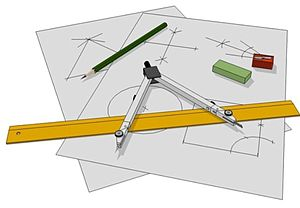
\includegraphics{Images/straight_edge_compass_wikipedia.jpg}
\end{center}

The ancient Greeks were curious about the following question which gave rise to these problems: Given a line segment of length 1 in the plane, 
for what values of $a$ can we construct a line segment of length $a$ using compass and straightedge constructions?

The Greeks discovered how to construct sums, differences, products, ratios, and square roots of given lengths. They could also construct half of a 
given angle; that is, they could ``bisect'' any angle. We will see these constructions below, and there are many other interesting constructions
they figured out.

However, there were some constructions they could not figure out. For example, they could not figure out how to trisect an arbitrary angle. That is, they could
not construct one third of a given angle except in some particular cases. They could not ``square a circle.'' That is, they could not figure out how to 
construct a square with the same area as a given circle.  Nor could they ``double a cube.'' That is, they could not figure out how to construct the 
side of a cube whose volume would be twice the volume of a cube with a given side.

The interest in these problems from our point of view is that it took the development of the theory of fields to solve these problems. In 1837 a
mathematician named Pierre Wantzel published a proof of the impossibility of trisecting an arbitrary angle or of doubling the volume of a cube, based on the 
impossibility of constructing cube roots of lengths. Then in 1882 Lindemann showed that $\pi$ is a transcendental number, and thus that it is impossible by 
straightedge and compass to construct a square with the same area as a given circle. These proofs are beautiful uses of the theory of fields, and we will
explore them below.

\subsection{The Rules of the Game}

In the past, compasses were used in mathematics, drafting, navigation and other purposes. Physical compasses are usually made of metal or 
plastic, and consist of two parts connected by a hinge which can be adjusted to allow the changing of the radius of the circle drawn. Typically 
one part has a spike at its end, and the other part a pencil or pen. Unlike physical compasses, we will assume our compasses can be opened arbitrarily 
wide. We will also assume that our compasses have no markings on them to measure angles or anything else. 

We will assume our straightedges are infinitely long, and has no markings on them. Our straightedges can only be used to draw a line segment between 
two points or to extend an existing segment.  

Our constructions must be exact. Sometimes you'll be tempted to ``eyeball'' it by looking at the construction and guessing at its accuracy, 
or using some form of measurement, such as the units of measure on a ruler. This is forbidden, and getting close does not count as a solution.

Compass and striaightedge construction must terminate. That is, they must have a finite number of steps, and cannot be the limit of ever closer 
approximations.

\subsection{The Fundamental Constructions}

\begin{definition}[Fundamental Constructions] The following compass and straightedge constructions are known as our three fundamental constructions.
  \begin{enumerate}
    \item Given two points, we may draw a line through them, extending it indefinitely in each direction.
    \item Given two points, we may draw the line segment connecting them.
    \item Given a point and line segment, we may draw a circle with center at the point and radius equal to the length of the line segment.
  \end{enumerate}
\end{definition}

\begin{example}
  Using the fundamental constructions, we can bisect any angle.
\end{example}

\begin{example}
  Using the fundamental constructions, we can construct angles of $30^\circ$ and $60^\circ$.
\end{example}

\begin{example}
  Using the fundamental constructions, we can draw a line parallel to a given line through any point not on the given line.
\end{example}

\subsection{Constructible Lengths}

\begin{lemma}
  Given segments of length 1, $a$ and $b$, it is possible to construct segments of lengths $a+b$, $a-b$ (when $a>b$), $ab$, and $a/b$.
  \label{lemma: rational constructions}
\end{lemma}

\begin{definition}
  A real number $a$ is constructible if given initially a segment of length $1$, it is possible to construct a segment of length $|a|$.
\end{definition}

\begin{lemma}
  Given segments of length $1$ and $a$, a segment of length $\sqrt{a}$ may be constructed.
  \label{lemma: sqrt can be constructed}
\end{lemma}

\subsection{Quadratic Extensions}

\begin{theorem}
  If $\mathbb{F}$ is a field, then so is $\mathbb{F}(\sqrt{k})$.
  \label{theorem: quadratic extensions of fields are fields}
\end{theorem}

\begin{theorem}
  A number $a$ is constructible if there is a finite sequence of fields $\mathbb{Q} = \mathbb{F}_0 \subset \mathbb{F}_1\subset \dots \subset \mathbb{F}_N$ with
  $a\in\mathbb{F}_N$ and such that for each $j$, $0\leq j \leq N-1$, $\mathbb{F}_{j+1}$ is a quadratic extension of $\mathbb{F}_j$.
  \label{theorem: constructible if in sequence of quadratic extensions}
\end{theorem}

\begin{definition}
  If $\mathbb{F}$ is a field, the plane of $\mathbb{F}$ will denote the set of all points $(x,y)$ in the Cartesian plane so that $x$ and $y$ are in $\mathbb{F}$. By a line in
  $\mathbb{F}$ we mean a line passing through two points in the plane of $\mathbb{F}$. By a circle in $\mathbb{F}$ we mean a circle with both its center and some point on its
  circumference in the plane of $\mathbb{F}$.
\end{definition}

Note that any fundamental construction using only points in the plane of a field $\mathbb{F}$ involves the construction of a line or a cube in $\mathbb{F}$.
TODO: Show this for a circle

\begin{lemma}
  Every line in $\mathbb{F}$ can be represented by an equation of the form $ax+by+c = 0$ with $a,b,c\in\mathbb{F}$
  \label{lemma: line in F}
\end{lemma}

\begin{lemma}
  Every circle in $\mathbb{F}$ can be represented by an equation of the form $x^2 + y^2 + ax + by +c = 0$ with $a,b,c\in\mathbb{F}$.
  \label{lemma: circle in F}
\end{lemma}

\begin{theorem}
  \begin{enumerate}
    \item The point of intersection of two distinct, nonparallel lines in $\mathbb{F}$ is in the plane of $\mathbb{F}$.
    \item The points of intersection of a line in $\mathbb{F}$ and a circle in $\mathbb{F}$ are either in the plane of $\mathbb{F}$
      or in the plane of some quadratic extension of $\mathbb{F}$.
    \item The points of intersection of two circles in $\mathbb{F}$ are either in the plane of $\mathbb{F}$
      or in the plane of some quadratic extension of $\mathbb{F}$.
  \end{enumerate}
  \label{theorem: intersections}
\end{theorem}

\begin{theorem}
  The following statements are equivalent:
  \begin{enumerate}
    \item The number $a$ is constructible.
    \item There is a finite sequence of fields $\mathbb{Q} = \mathbb{F}_0 \subset \mathbb{F}_1\subset \dots \subset \mathbb{F}_N$ with
  $a\in\mathbb{F}_N$ and such that for each $j$, $0\leq j \leq N-1$, $\mathbb{F}_{j+1}$ is a quadratic extension of $\mathbb{F}_j$.
  \end{enumerate}<++>
  \label{theorem: constructible iff in sequence of quadratic extensions}
\end{theorem}

\section{Three Famous Problems}

\subsection{Doubling the Cube}

Given a line segment representing the edge of a cube, is it possible to construct another line segment representing the edge of a cube with exactly
twice the volume of the first cube?

Without loss of generality we will take the length of a side of the original cube to be 1. Then the desired line segment must have length $\sqrt[3]{2}$.

\begin{theorem}
  Let $\mathbb{F}(\sqrt{k})$ be a quadratic extension of a field $\mathbb{F}$. If $\sqrt[3]{2}$ is in $\mathbb{F}(\sqrt{k})$, then $\sqrt[3]{2}$ must be in $\mathbb{F}$ itself.
  \label{theorem: cube root of 2}
\end{theorem}

\begin{theorem}
  It is impossible to double the cube.
  \label{theorem: can't double cube}
\end{theorem}

\subsection{Trisecting an Angle}

TODO: We show that it is impossible to trisect an angle of $60^\circ$. If this were possible, it would be possible to construct a $20^\circ$ angle. This implies that $\cos(20^\circ)$ is constructible.
This implies that a root of $x^3-3x  -1 =0$ is constructible.

\begin{theorem}
  If $\mathbb{F}(\sqrt{k})$ contains a root of $x^2-3x-1=0$, then so does $\mathbb{F}$.
  \label{theorem: trisecting set up}
\end{theorem}

\begin{theorem}
  It is not possible to trisect and arbitrary angle.
  \label{theorem: can't trisect arbitrary angle}
\end{theorem}

\subsection{Squaring a Circle}


\end{document}



